\documentclass[12pt,a4paper]{report}
\usepackage[left=1.50cm, right=2.00cm, top=2.00cm, bottom=2.00cm]{geometry} % Tùy chỉnh lề
\usepackage{mathpazo} % Gói dùng để thay đổi phông chữ mặc định của tài liệu sang phông Palatino, và cung cấp phông chữ tương thích cho các ký hiệu toán học
\usepackage{graphicx} % Gói để chèn và xử lý hình ảnh: \includegraphics[cấu hình]{tên file} 
\usepackage[utf8]{vietnam} % Gói lệnh để gõ tiếng việt
\usepackage{amsmath, amssymb} % Gói lệnh toán học
\usepackage{amsfonts} % Gói dùng để mở rộng các ký hiệu toán học, đặc biệt là các ký hiệu tập hợp và phông chữ toán học đặc biệt
\usepackage{array} % Gói lệnh thêm các chức năng mở rộng cho bảng 
\usepackage{hhline} % Gói lệnh cải tiến hline: - một gạch ngang, = hai gạch ngang, ~ trống gạch ngang, # hai gạch xuống cắt qua hai gạch ngang, | một gạch xuống
\usepackage{xcolor} % Gói tùy chỉnh màu sắc: \textcolor{màu}{Văn bản}, \colorbox{màu}{Văn bản}, \fcolorbox{màu 1}{màu 2}{Văn bản}, \definecolor{tên màu mới}{mô hình màu sắc}{thông số màu}
\usepackage{listings} % Gói dùng để hiển thị mã nguồn (code) chuyên nghiệp và có tô màu cú pháp trong tài liệu
\usepackage{fancyhdr} % Gói dùng để tùy chỉnh header (đầu trang) và footer (chân trang) của tài liệu
\usepackage[hidelinks]{hyperref} % Gói tạo liên kết trong và ngoài tài liệu
\usepackage{tikz} % Gói để vẽ hình ảnh vector, sơ đồ, biểu đồ, hình học, hình minh họa, sơ đồ khối, cây phân cấp, đồ thị mạng,...
\usetikzlibrary{shapes.geometric, arrows} % Dùng để nạp thêm thư viện con cho TikZ, giúp vẽ các sơ đồ khối (flowchart) hoặc các hình học đặc biệt.
\definecolor{fitblue}{RGB}{0, 80, 150} % Mã màu gần giống với logo
\usepackage{tocloft}
\renewcommand{\cfttoctitlefont}{\LARGE\bfseries} % căn giữa và đổi kích thước
\setlength{\cftbeforetoctitleskip}{0pt}
\setlength{\cftaftertoctitleskip}{0pt}\usepackage{xcolor}     % Cho màu sắc
\usepackage{etoolbox}   % Cho phép chỉnh sửa môi trường LaTeX

\makeatletter
\renewcommand{\@cite}[2]{\textcolor{blue}{[#1\if@tempswa , #2\fi]}}
\makeatother

%------Gói lệnh hỗ trợ bảng------ 
\usepackage{multirow} % Gộp hàng
\usepackage{multicol} % Gộp cột
\usepackage{booktabs} % Tùy chỉnh bảng đẹp hơn
\usepackage{colortbl} % Thêm màu
\usepackage{longtable} % Kéo dài bảng qua các trang
\usepackage{fancybox}
\usepackage{setspace}
\usepackage{booktabs}
\usepackage{float}
%------Định nghĩa kiểu cột có khả năng tùy chỉnh kích thước-----
\newcolumntype{L}[1]{>{\raggedright\let\newline\\\arraybackslash\hspace{0pt}}m{#1}}
\newcolumntype{C}[1]{>{\centering\let\newline\\\arraybackslash\hspace{0pt}}m{#1}}
\newcolumntype{R}[1]{>{\raggedleft\let\newline\\\arraybackslash\hspace{0pt}}m{#1}}
%------Định nghĩa listings C++------
\lstset{
    frame=single,
    language=C++,
    aboveskip=3mm,
    belowskip=3mm,
    showstringspaces=false,
    columns=flexible,
    basicstyle={\normalsize\ttfamily},
    numbers=none, % Không hiển thị số dòng
    keywordstyle=\color{blue},
    commentstyle=\color{dkgreen},
    stringstyle=\color{mauve},
    breaklines=true,
    breakatwhitespace=true,
    tabsize=3
} 
\lstdefinestyle{numbered}{ % Style cho code có đánh số
    numbers=left, % Hiển thị số dòng bên trái
    numberstyle=\small\color{gray},
    numbersep=5pt, % Khoảng cách giữa số dòng và mã nguồn
    frame=single,
    framexleftmargin=15pt, % Đẩy khung bao quanh để chứa số dòng
    xleftmargin=15pt, % Lề trái để số dòng không bị cắt
    language=C++,
    aboveskip=3mm,
    belowskip=3mm,
    showstringspaces=false,
    columns=flexible,
    basicstyle={\normalsize\ttfamily},
    keywordstyle=\color{blue},
    commentstyle=\color{dkgreen},
    stringstyle=\color{mauve},
    breaklines=true,
    breakatwhitespace=true,
    tabsize=3
}
\begin{document}

\thispagestyle{empty}
\begin{center}
\thispagestyle{empty}  % Không đánh số
    \setlength{\fboxrule}{1.2pt}
    \doublebox{%
        \begin{minipage}{0.95\textwidth}
            \begin{center}
                \vspace{0.6cm}
                ĐẠI HỌC QUỐC GIA THÀNH PHỐ HỒ CHÍ MINH\\
                TRƯỜNG ĐẠI HỌC KHOA HỌC TỰ NHIÊN\\
                \textbf{KHOA CÔNG NGHỆ THÔNG TIN}\\[0.4em]
                -\hspace{0.01cm}-\hspace{0.01cm}-\hspace{0.01cm}-\hspace{0.01cm}-\hspace{0.01cm}-\textbf{oOo}-\hspace{0.01cm}-\hspace{0.01cm}-\hspace{0.01cm}-\hspace{0.01cm}-\hspace{0.01cm}-\\[2em]

                % Logo
                
\includegraphics[width=0.20\textwidth]{logo-hcmus.png}\\[1em]

                \textbf{\LARGE BÁO CÁO ĐỒ ÁN MÔN HỌC}\\[0.5em]
                \textbf{CSC10004 - Cấu Trúc Dữ Liệu Và Giải Thuật}\\[1em]
                \textcolor{fitblue}{\LARGE{\textbf{NGHIÊN CỨU VÀ ĐÁNH GIÁ HIỆU NĂNG PHƯƠNG PHÁP DOUBLE HASHING \\TRONG BẢNG BĂM}}}\\[5em]

                \begin{tabular}{ l  l }
                    \textbf{Giảng viên hướng dẫn}  &: CN. Lê Nhựt Nam \\
                    \textbf{Nhóm sinh viên thực hiện} &: Nhóm 9 -- Lớp 24CTT2A \\
                \end{tabular}\\[1.5em]

                % Bảng thành viên
                \renewcommand{\arraystretch}{1.2}
                \begin{tabular}{ c  l  c }
                
                    \textbf{STT} & \textbf{Họ và tên} & \textbf{MSSV} \\
                    
                    1 & Trương Tuấn Anh & 24120260 \\
                    2 & Tôn Thất Kiên & 24120078 \\
                    3 & Bùi Văn Thiên & 24120138 \\
                    4 & Bùi Trọng An & 24120252 \\
                
                \end{tabular}
                
                \vspace{11em}
                \textbf{TP. Hồ Chí Minh, tháng 6 năm 2025}
                \\[3em]
                \textbf{ }
            \end{center}
        \end{minipage}
    }
\end{center}

\newpage
\pagenumbering{arabic}
\setcounter{page}{1}

\chapter*{\centering{LỜI CAM KẾT}}
\addcontentsline{toc}{chapter}{\textcolor{fitblue}{LỜI CAM KẾT}}

\setlength{\parindent}{2em}   % Thụt đầu dòng mỗi đoạn
\setlength{\parskip}{0.5em}     % Dãn đoạn giữa các đoạn văn

\noindent \indent Nhóm chúng em xin cam kết rằng đồ án “\textit{Nghiên cứu và đánh giá hiệu năng phương pháp Double Hashing trong bảng băm}” là công trình do chính nhóm thực hiện dưới sự hướng dẫn của giảng viên hướng dẫn.

\textbf{\textit{Về tính độc lập và nguyên gốc:}}

- Toàn bộ nội dung nghiên cứu, phân tích và triển khai trong báo cáo đều do nhóm tự thực hiện, không sao chép từ bất kỳ nguồn nào một cách không hợp lệ.

- Các kết quả, thuật toán, biểu đồ, và đoạn mã nguồn (code implementation) đều được xây dựng và kiểm chứng trong quá trình học tập và nghiên cứu của các thành viên trong nhóm.

- Nhóm cam kết không sử dụng toàn bộ hoặc một phần nội dung từ các báo cáo, đồ án, tài liệu của người khác mà không có sự cho phép hoặc không trích dẫn rõ ràng.

\textbf{\textit{Về tài liệu tham khảo:}}

- Mọi tài liệu, dữ liệu và nguồn thông tin được sử dụng trong quá trình thực hiện đều được trích dẫn và ghi nguồn rõ ràng, đúng quy định học thuật.

- Các thuật toán, mô hình phân tích được tham khảo từ các tài liệu học thuật uy tín, đồng thời kết hợp với kiến thức tích lũy trong quá trình học tập tại trường.

- Tất cả ý tưởng, quan điểm không phải của nhóm đều được ghi nhận và dẫn nguồn cụ thể theo chuẩn học thuật.

\textbf{\textit{Về trách nhiệm:}}

- Nhóm hoàn toàn chịu trách nhiệm về tính chính xác và trung thực của toàn bộ nội dung báo cáo.

- Trong trường hợp có phát hiện sai sót, nhóm cam kết sẽ chủ động tiếp nhận và khắc phục kịp thời.

- Nhóm cam kết tuân thủ đầy đủ các quy định về đạo đức học thuật và nghiên cứu khoa học của khoa và nhà trường.

\begin{flushright}
TP. Hồ Chí Minh, tháng 6 năm 2025\\
Đại diện nhóm thực hiện \\
\end{flushright}

\chapter*{\centering{LỜI MỞ ĐẦU}}
\addcontentsline{toc}{chapter}{\textcolor{fitblue}{LỜI MỞ ĐẦU}}
\noindent \indent Trong hành trình tiếp cận và chinh phục những nền tảng cốt lõi của khoa học máy tính, học phần \textit{Cấu trúc dữ liệu và giải thuật} đã mang đến cho nhóm nhiều trải nghiệm sâu sắc. Trong đó, kỹ thuật xử lý va chạm trong bảng băm nổi bật lên như một chủ đề vừa giàu tính học thuật, vừa có tính ứng dụng cao trong các bài toán tối ưu lưu trữ và truy xuất dữ liệu.

Xuất phát từ sự hứng thú và tinh thần khám phá, nhóm đã chọn đề tài:
“\textit{Nghiên cứu và đánh giá hiệu năng phương pháp Double Hashing trong bảng băm}” làm hướng đi chính cho đồ án lần này.

Đây không chỉ là cơ hội để nhóm vận dụng kiến thức lý thuyết vào thực tiễn mà còn là dịp để rèn luyện tư duy logic, kỹ năng lập trình, phân tích và đánh giá thuật toán một cách có hệ thống. Quá trình thực hiện đề tài cũng là một thử thách thực sự, khi nhóm phải đối mặt với nhiều khó khăn: từ xử lý dữ liệu, tối ưu hóa mã nguồn cho đến việc trình bày và trực quan hóa kết quả. Tuy nhiên, với sự hướng dẫn tận tình và hỗ trợ quý báu từ thầy CN. Lê Nhựt Nam, nhóm đã từng bước tháo gỡ vướng mắc và hoàn thành đề tài với nhiều bài học đáng giá.

Nhóm xin chân thành cảm ơn thầy, người không chỉ truyền đạt kiến thức chuyên môn mà còn truyền cảm hứng và đồng hành cùng nhóm trong suốt quá trình thực hiện đồ án.

Dẫu đã nỗ lực hết mình, nhóm ý thức rằng báo cáo vẫn còn nhiều mặt hạn chế. Rất mong nhận được những ý kiến đóng góp và nhận xét từ thầy cũng như các bạn để nhóm có thể hoàn thiện hơn trong những lần nghiên cứu tiếp theo.

\vspace{2em}

\begin{flushright}
TP. Hồ Chí Minh, tháng 6 năm 2025\\
Nhóm sinh viên thực hiện
\end{flushright}




\renewcommand{\contentsname}{}        % Xóa "Mục lục"
\renewcommand{\listtablename}{}       % Xóa "Danh mục các bảng"
\renewcommand{\listfigurename}{}      % Xóa "Danh mục hình vẽ"

% MỤC LỤC
\chapter*{\centering{MỤC LỤC}}
\addcontentsline{toc}{chapter}{\textcolor{fitblue}{MỤC LỤC}}
\tableofcontents

% DANH MỤC BẢNG
\newpage
\chapter*{\centering{\MakeUppercase{Danh mục các bảng}}}
\vspace*{-7em}
\addcontentsline{toc}{chapter}{\textcolor{fitblue}{\MakeUppercase{Danh mục các bảng}}}
\listoftables

% DANH MỤC HÌNH VẼ
\newpage
\chapter*{\centering{\MakeUppercase{Danh mục các hình vẽ, đồ thị}}}
\vspace*{-7em}
\addcontentsline{toc}{chapter}{\textcolor{fitblue}{\MakeUppercase{Danh mục các hình vẽ, đồ thị}}}
\listoffigures

\newpage
\chapter*{\centering{\MakeUppercase{Chương I. Giới thiệu}}}
\addcontentsline{toc}{chapter}{\textcolor{fitblue}{\MakeUppercase{Chương I. Giới thiệu}}}

\section*{1.1. Bối cảnh và lý do chọn đề tài}
\addcontentsline{toc}{section}{{1.1. Bối cảnh và lý do chọn đề tài}}
\noindent \indent Sự phát triển nhanh chóng của công nghệ thông tin và dữ liệu lớn (big data) đã đặt ra yêu cầu ngày càng cao đối với hiệu quả lưu trữ và truy xuất thông tin trong các hệ thống phần mềm. Trong bối cảnh đó, việc thiết kế và lựa chọn cấu trúc dữ liệu phù hợp đóng vai trò then chốt trong việc đảm bảo hiệu năng hệ thống, đặc biệt đối với các thao tác tìm kiếm và ánh xạ khóa.

Bảng băm (hash table) là một trong những cấu trúc dữ liệu nền tảng, được ứng dụng rộng rãi nhờ khả năng hỗ trợ truy xuất với độ phức tạp trung bình gần như hằng số. Tuy nhiên, hiệu quả của bảng băm bị ảnh hưởng đáng kể bởi hiện tượng va chạm khóa (collision) – khi nhiều khóa được ánh xạ tới cùng một chỉ số trong bảng. Việc xử lý va chạm không hiệu quả có thể làm suy giảm đáng kể hiệu suất truy xuất, đặc biệt khi hệ số tải cao hoặc phân phối khóa không đều.

Trong số các kỹ thuật xử lý va chạm thuộc nhóm địa chỉ mở (open addressing), Double Hashing được đánh giá cao nhờ khả năng giảm thiểu hiện tượng kết cụm (clustering) và cung cấp chuỗi dò tìm có tính phân tán cao. Mặc dù đã được đề cập trong nhiều tài liệu học thuật, hiệu quả thực tế của Double Hashing vẫn phụ thuộc vào lựa chọn hàm băm, hệ số tải và đặc điểm của tập dữ liệu.

Từ những lý do trên, nhóm lựa chọn đề tài:
“\textit{Nghiên cứu và đánh giá hiệu năng phương pháp Double Hashing trong bảng băm}”
nhằm khảo sát, hiện thực và đánh giá định lượng hiệu quả của kỹ thuật này trong các điều kiện khác nhau, từ đó rút ra các khuyến nghị về ứng dụng thực tiễn.

\section*{1.2. Lược sử về bảng băm và kỹ thuật Double Hashing}
\addcontentsline{toc}{section}{{1.2. Lược sử về bảng băm và kỹ thuật Double Hashing}}
\noindent \indent Bảng băm (\textit{hash table}) là một trong những cấu trúc dữ liệu nền tảng và có ảnh hưởng sâu rộng trong khoa học máy tính, đặc biệt trong lĩnh vực lưu trữ và truy xuất dữ liệu hiệu quả. Khái niệm sử dụng hàm băm để ánh xạ khóa về vị trí lưu trữ trong bảng được đề xuất sớm nhất vào năm 1953 bởi \textbf{Hans Peter Luhn} tại IBM trong bối cảnh xử lý thông tin tự động~\cite{luhn1953}. Tuy nhiên, mãi đến cuối thập niên 1960, kỹ thuật băm mới được phát triển một cách hệ thống như một cấu trúc dữ liệu chủ đạo.

Năm 1968, \textbf{Donald Knuth} đã đưa khái niệm và phân tích kỹ thuật bảng băm vào tập đầu tiên của bộ sách \textit{The Art of Computer Programming}, qua đó đặt nền móng lý thuyết cho các phương pháp băm hiện đại~\cite{knuth1998}. Bảng băm cho phép truy xuất dữ liệu với độ phức tạp trung bình gần như hằng số $O(1)$, điều này làm cho nó trở thành lựa chọn phổ biến trong các hệ thống yêu cầu hiệu năng cao như trình biên dịch, bộ nhớ đệm, cơ sở dữ liệu và máy học.

Tuy nhiên, một trong những vấn đề kỹ thuật lớn nhất khi sử dụng bảng băm là hiện tượng \textbf{va chạm khóa} (\textit{collision}) – xảy ra khi nhiều khóa được ánh xạ tới cùng một chỉ số trong bảng. Để giải quyết, hai nhóm kỹ thuật chính được phát triển: \textit{liên kết ngoài (chaining)} và \textit{địa chỉ mở (open addressing)}. Trong nhóm địa chỉ mở, nhiều chiến lược dò tìm đã được nghiên cứu, gồm:

- \textbf{Linear probing}: dò từng bước liên tiếp.

- \textbf{Quadratic probing}: dò với bước nhảy tăng dần theo bình phương.

- \textbf{Double hashing}: sử dụng hàm băm thứ hai để xác định bước nhảy.

\textbf{Double Hashing} được mô tả chính thức lần đầu bởi Knuth vào năm 1973 trong tập III của \textit{The Art of Computer Programming}~\cite{knuth1998}. Phương pháp này tạo ra chuỗi dò có dạng:
\[
h(k, i) = (h_1(k) + i \cdot h_2(k)) \mod m
\]
Trong đó $h_1(k)$ và $h_2(k)$ là hai hàm băm độc lập, giúp giảm hiện tượng kết cụm (\textit{clustering}) – nhược điểm phổ biến của linear và quadratic probing.

Về mặt lý thuyết, \textbf{Carter và Wegman (1979)} đã chứng minh rằng nếu $h_2(k)$ được chọn sao cho $\gcd(h_2(k), m) = 1$, thì chuỗi dò sẽ bao phủ toàn bộ bảng mà không bị lặp, tương đương với một lớp hàm băm phổ quát (\textit{universal class of hash functions})~\cite{carter1979}. Điều này cho phép Double Hashing đạt hiệu năng gần tương đương với \textit{uniform hashing} – chiến lược lý tưởng sử dụng vô hạn hàm băm độc lập – nhưng với chi phí thực thi thấp hơn nhiều.

Trong các nghiên cứu thực nghiệm, \textbf{Brent (1973)} đã chỉ ra rằng số lần dò trung bình khi sử dụng Double Hashing có thể được xấp xỉ bởi công thức:
\[
\overline{C}_\alpha \approx \frac{1}{1 - \alpha}
\]
với $\alpha$ là hệ số tải của bảng băm~\cite{brent1973}. Công thức này từng được xem là đặc trưng của phương pháp \textit{uniform probing}, nhưng đáng chú ý là Double Hashing – chỉ sử dụng hai hàm băm – vẫn đạt kết quả gần tương đương trong nhiều trường hợp.

Nhờ sự đơn giản, hiệu quả và khả năng tổng quát hóa tốt, Double Hashing hiện vẫn được sử dụng trong nhiều thư viện lập trình hiện đại như C++, Java, Python, cũng như trong các hệ thống cơ sở dữ liệu, máy ảo và bộ nhớ phân tán.

\section*{1.3. Khoảng trống nghiên cứu}
\addcontentsline{toc}{section}{{1.3. Khoảng trống nghiên cứu}}
\noindent \indent Mặc dù kỹ thuật Double Hashing đã được trình bày trong nhiều tài liệu kinh điển và áp dụng rộng rãi trong thực tiễn, phần lớn các phân tích hiện có chủ yếu tập trung vào khía cạnh lý thuyết hoặc đánh giá hiệu năng trong điều kiện lý tưởng – với dữ liệu đầu vào ngẫu nhiên và hàm băm phân phối đều. Trong môi trường thực tế, khóa thường không phân bố đồng đều, hệ số tải có thể biến động lớn, và việc chọn hàm băm phù hợp trở nên phức tạp hơn.

Bên cạnh đó, nhiều công trình nghiên cứu vẫn còn thiếu các phân tích định lượng chi tiết về hiệu năng của Double Hashing trong các kịch bản cụ thể, ví dụ như:

- So sánh trực tiếp với Linear và Quadratic Probing trên cùng một bộ dữ liệu.

- Đánh giá ảnh hưởng của hệ số tải (load factor) đến độ dài chuỗi dò (probe length), thời gian tìm kiếm và độ phức tạp tổng thể.

- Phân tích hiệu quả khi áp dụng kỹ thuật này với các tập khóa có tính chất cụm, tuần tự, hoặc lệch phân phối – vốn thường gặp trong cơ sở dữ liệu thực tế.

Chính vì vậy, vẫn tồn tại khoảng trống đáng kể trong việc kiểm chứng thực nghiệm và hệ thống hóa các yếu tố ảnh hưởng đến hiệu năng thực tế của Double Hashing, từ đó đưa ra các khuyến nghị ứng dụng phù hợp.

\section*{1.4. Mục tiêu và nhiệm vụ nghiên cứu}
\addcontentsline{toc}{section}{{1.4. Mục tiêu và nhiệm vụ nghiên cứu}}
\subsection*{1.4.1. Mục tiêu nghiên cứu}
\noindent \indent \textbf{\textit{Nghiên cứu này hướng đến việc:}}

- Hiện thực và triển khai thuật toán Double Hashing trong bảng băm sử dụng phương pháp địa chỉ mở.

- Thiết kế các kịch bản thí nghiệm đa dạng để đánh giá hiệu năng thuật toán trong điều kiện thực tế và so sánh với các kỹ thuật dò tìm phổ biến khác (Linear và Quadratic Probing).

- Phân tích mối quan hệ giữa hệ số tải, đặc tính bộ dữ liệu và hiệu suất thực thi của Double Hashing.

- Rút ra các kết luận và khuyến nghị về việc áp dụng Double Hashing trong thiết kế hệ thống lưu trữ và truy xuất hiệu quả.
\subsection*{1.4.2. Nhiệm vụ nghiên cứu}
\noindent \indent \textbf{\textit{Để đạt được các mục tiêu trên, đề tài tập trung thực hiện các nhiệm vụ sau:}}

- Tổng quan lý thuyết về bảng băm, các kỹ thuật xử lý va chạm, và nguyên lý hoạt động của Double Hashing.

- Thiết kế và cài đặt mô hình bảng băm sử dụng ba kỹ thuật dò tìm: Linear Probing, Quadratic Probing và Double Hashing.

- Xây dựng bộ dữ liệu thử nghiệm với nhiều dạng phân phối khác nhau (ngẫu nhiên, tuần tự, cụm) và thiết lập các mức hệ số tải khác nhau.

- Đo lường và phân tích các chỉ số hiệu năng, bao gồm:

\hspace{1cm}+ Số phép dò trung bình khi chèn và tìm kiếm khóa.

\hspace{1cm}+ Thời gian thực thi của từng kỹ thuật.

\hspace{1cm}+ Độ dài cụm và độ phân tán khóa.

- Trình bày kết quả dưới dạng trực quan hóa và phân tích định lượng để so sánh, đối chiếu giữa các kỹ thuật.

- Đề xuất ứng dụng thực tiễn và định hướng cải tiến thuật toán trong các bối cảnh hệ thống khác nhau.

\section*{1.5. Đối tượng và phạm vi nghiên cứu}
\addcontentsline{toc}{section}{{1.5. Đối tượng và phạm vi nghiên cứu}}
\subsection*{1.5.1. Đối tượng nghiên cứu}
\noindent \indent Đối tượng nghiên cứu của đề tài là \textbf{kỹ thuật Double Hashing} trong cấu trúc \textit{bảng băm sử dụng địa chỉ mở} (open addressing hash table), với trọng tâm là:

    - Nguyên lý hoạt động và công thức áp dụng của kỹ thuật Double Hashing.
    
    - Hiệu năng của Double Hashing khi xử lý va chạm trong bảng băm.
    
    - Các yếu tố ảnh hưởng đến hiệu quả thực thi của thuật toán, bao gồm hệ số tải, đặc điểm phân phối dữ liệu và lựa chọn hàm băm.

Ngoài ra, đề tài cũng nghiên cứu \textit{so sánh hiệu năng thực nghiệm} giữa Double Hashing và hai kỹ thuật dò tìm phổ biến khác là Linear Probing và Quadratic Probing, trên cùng tập dữ liệu và môi trường thực thi.

\subsection*{1.5.2. Phạm vi nghiên cứu}

\noindent \indent Phạm vi nghiên cứu của đề tài được giới hạn như sau:

    - Nghiên cứu chỉ tập trung vào bảng băm với địa chỉ mở; không xét các kỹ thuật xử lý va chạm bằng danh sách liên kết (chaining).
    
    - Chỉ xét các hàm băm tuyến tính và dạng mô đun: $h_1(k) = k \mod m$, $h_2(k) = R - (k \mod R)$, với $R < m$ là số nguyên tố.
    
    - Thí nghiệm đánh giá hiệu năng được thực hiện trên môi trường giả lập cục bộ, với ba kiểu dữ liệu đầu vào: ngẫu nhiên, tuần tự và cụm (clustered), nhằm mô phỏng các tình huống thực tế thường gặp. Tập dữ liệu đầu vào bao gồm các kích thước: 1000, 5000, 10000, 15000, 20000, 25000, 30000, 35000, và 40000 phần tử. Hai mức hệ số tải được sử dụng trong thí nghiệm là: 0.5 và 0.8, nhằm đánh giá hiệu năng của bảng băm trong các tình huống tải khác nhau.
    
    - Các chỉ số hiệu năng được đo lường bao gồm: số lần dò trung bình khi chèn và tìm kiếm, thời gian thực thi, và độ phân tán trong bảng.
    
    - Không đi sâu vào tối ưu hóa phần cứng hoặc các vấn đề hệ thống phân tán; không sử dụng thư viện hàm băm hệ thống hoặc thuật toán mã hóa chuyên biệt.


\section*{1.6. Phương pháp nghiên cứu}
\addcontentsline{toc}{section}{{1.6. Phương pháp nghiên cứu}}

\noindent \indent Để đạt được mục tiêu nghiên cứu đã đề ra, đề tài kết hợp giữa phương pháp \textbf{nghiên cứu tài liệu}, \textbf{thực nghiệm mô phỏng} và \textbf{phân tích định lượng}. Cách tiếp cận này đảm bảo đề tài vừa có nền tảng lý thuyết vững chắc, vừa phản ánh đúng hiệu năng thực tiễn của các thuật toán xử lý va chạm trong bảng băm.

\subsection*{1.6.1. Phương pháp nghiên cứu lý thuyết}
    \noindent \indent- Tổng quan và hệ thống hóa kiến thức từ các tài liệu học thuật uy tín (Knuth, Cormen, Carter \& Wegman…) về bảng băm, kỹ thuật địa chỉ mở, và các chiến lược dò tìm như Linear Probing, Quadratic Probing, và Double Hashing.
    
    - Phân tích đặc điểm lý thuyết của các thuật toán: công thức dò tìm, điều kiện đảm bảo tính đầy đủ dãy dò, hành vi khi thay đổi hệ số tải, và các giả định phân phối khóa.
    
    - Trích xuất mô hình hiệu năng dựa trên số lần probe trung bình (theoretical expected probes), từ đó làm cơ sở để đối chiếu với kết quả thực nghiệm.

\subsection*{1.6.2. Phương pháp thực nghiệm}
    \noindent \indent - Xây dựng chương trình mô phỏng bảng băm sử dụng ba kỹ thuật dò: Linear Probing, Quadratic Probing và Double Hashing bằng ngôn ngữ lập trình C++.
    
    - Thiết kế bộ dữ liệu đầu vào với ba kiểu phân phối khóa:
    
        \hspace{1cm}+ Ngẫu nhiên hoàn toàn (uniform random)
        
       \hspace{1cm}+ Tuần tự tăng (sequential)
       
        \hspace{1cm}+ Cụm hóa (clustered)
 
    - Đặt hệ số tải (load factor) ở mức thấp (0.5) và mức sát ngưỡng đầy (0.8) để quan sát ảnh hưởng đến hiệu năng.
    
    - Đo lường các chỉ số hiệu năng chính:

       \hspace{1cm}+ Số lần probe trung bình khi chèn và tìm kiếm
        
        \hspace{1cm}+ Thời gian thực thi cho mỗi thao tác
        
        \hspace{1cm}+ Mức độ kết cụm và khả năng phân tán khóa

\subsection*{1.6.3. Phân tích và trình bày kết quả}
    \noindent \indent - Trực quan hóa kết quả thông qua biểu đồ và bảng số liệu nhằm hỗ trợ so sánh hiệu năng giữa các kỹ thuật.
    
    - Phân tích định lượng và định tính: đánh giá ưu – nhược điểm của từng kỹ thuật dưới các điều kiện cụ thể.
    
    - Đối chiếu với lý thuyết: so sánh kết quả thực nghiệm với các mô hình lý thuyết để kiểm chứng giả thuyết ban đầu.

\subsection*{1.6.4. Công cụ và môi trường triển khai}

    \noindent \indent - Ngôn ngữ lập trình: C++ (chuẩn C++17).
    
    - IDE và công cụ biên dịch: Visual Studio Code, GCC/G++.
    
    - Thư viện hỗ trợ: \texttt{chrono} (đo thời gian), \texttt{random} (sinh dữ liệu).
    
   - Hệ điều hành: Windows 11.

\section*{1.7. Cấu trúc và kế hoạch thực hiện báo cáo}
\addcontentsline{toc}{section}{{1.7. Cấu trúc và kế hoạch thực hiện báo cáo}}
\subsection*{1.7.1. Cấu trúc báo cáo}
\noindent \indent Báo cáo được tổ chức thành 5 chương chính như sau:

- \textit{Chương I – Giới thiệu}: Trình bày bối cảnh, lý do chọn đề tài, khoảng trống nghiên cứu, mục tiêu – nhiệm vụ, phạm vi, phương pháp nghiên cứu và cấu trúc báo cáo.

-\textit{ Chương II – Tổng quan về kỹ thuật băm và phương pháp Double Hashing}: Hệ thống hóa cơ sở lý thuyết về bảng băm, vấn đề va chạm, các kỹ thuật dò địa chỉ (Linear, Quadratic, Double Hashing), và phân tích nguyên lý hoạt động của Double Hashing.

- \textit{Chương III – Cài đặt và đánh giá thực nghiệm}: Mô tả chi tiết quá trình thiết kế, xây dựng chương trình thử nghiệm, cấu hình thí nghiệm, cách thu thập dữ liệu và thống kê các chỉ số hiệu năng.

- \textit{Chương IV – Phân tích và đánh giá kết quả}: Trình bày kết quả thực nghiệm, phân tích định lượng các chỉ số như số phép dò, thời gian xử lý, độ kết cụm..., và so sánh giữa các kỹ thuật.

- \textit{Chương V – Kết luận và hướng phát triển}: Tổng kết những đóng góp chính, nêu rõ giới hạn của nghiên cứu, đồng thời đề xuất một số hướng mở rộng và ứng dụng thực tế trong tương lai.
\subsection*{1.7.2. Kế hoạch thực hiện}
\noindent \indent Quá trình thực hiện đề tài được chia thành 6 giai đoạn cụ thể như sau:
\begin{table}[H]
\centering
\renewcommand{\arraystretch}{1.3}
\begin{tabular}{|c|c|p{9cm}|}
\hline
\textbf{Giai đoạn} & \textbf{Thời gian} & \textbf{Nội dung công việc chính} \\
\hline
1 & Tuần 1–2 & Tìm hiểu đề tài, thu thập và tổng hợp tài liệu lý thuyết \\
\hline
2 & Tuần 3–4 & Thiết kế cấu trúc chương trình, cài đặt các thuật toán Linear, Quadratic và Double Hashing \\
\hline
3 & Tuần 5 & Thiết kế bộ dữ liệu thử nghiệm và công cụ đo hiệu năng \\
\hline
4 & Tuần 6–7 & Chạy mô phỏng, thu thập và xử lý kết quả thống kê \\
\hline
5 & Tuần 8 & Viết báo cáo, trình bày kết quả bằng biểu đồ và bảng số liệu \\
\hline
GĐ6 & Tuần 9 & Rà soát, chỉnh sửa, hoàn thiện báo cáo và chuẩn bị nội dung bảo vệ \\
\hline
\end{tabular}
\caption{Kế hoạch thực hiện đề tài}
\end{table}

\newpage
\chapter*{\centering{\MakeUppercase{Chương II. Tổng quan về kỹ thuật băm và phương pháp Double Hashing}}}
\addcontentsline{toc}{chapter}{\textcolor{fitblue}{\MakeUppercase{Chương II. Tổng quan về kỹ thuật băm và phương pháp Double Hashing}}}

\section*{2.1. Tổng quan về bảng băm}
\addcontentsline{toc}{section}{{2.1. Tổng quan về bảng băm}}
\noindent \indent Bảng băm (hash table) là một cấu trúc dữ liệu hiệu quả, cho phép lưu trữ và truy xuất các cặp khóa – giá trị (key–value) với thời gian trung bình gần như hằng số, tức là \texttt{O(1)} \cite{cormen2009}. Nguyên lý hoạt động của bảng băm dựa trên một hàm băm (hash function) có nhiệm vụ ánh xạ khóa đầu vào \texttt{k} tới một vị trí chỉ số trong bảng có kích thước \texttt{m}, thông qua công thức \texttt{h(k) = k mod m} hoặc các biến thể phù hợp với kiểu dữ liệu.

Cấu trúc bảng băm được ưa chuộng trong nhiều ứng dụng thực tiễn như từ điển ánh xạ, hệ thống tra cứu, kiểm tra trùng lặp, bộ nhớ đệm, và tối ưu thuật toán quy hoạch động. Tính ưu việt của bảng băm đến từ khả năng truy xuất trực tiếp, độc lập với kích thước dữ liệu, miễn là hàm băm được thiết kế tốt và phân phối đồng đều.

Tuy nhiên, một trong những thách thức cốt lõi của bảng băm là hiện tượng va chạm (collision), xảy ra khi hai khóa khác nhau cùng được ánh xạ tới một vị trí trong bảng. Hiện tượng này là không thể tránh khỏi, đặc biệt khi không gian khóa lớn hơn không gian bảng lưu trữ.
\begin{quote}
“Hash tables are among the most efficient data structures for fast access when the number of keys is large and key distribution is unpredictable.”
(\textit{Cormen, Leiserson, Rivest, \& Stein, 2009, trang 257}) \\
(Tạm dịch: Bảng băm là một trong những cấu trúc dữ liệu hiệu quả nhất để truy xuất nhanh khi số lượng khóa lớn và phân phối khóa không thể đoán trước được.)
\end{quote}
\section*{2.2. Vấn đề va chạm trong bảng băm}
\addcontentsline{toc}{section}{{2.2. Vấn đề va chạm trong bảng băm}}
\noindent \indent Va chạm là tình huống xảy ra khi \texttt{h($k_1$) = h($k_2$)} trong khi \texttt{$k_1 \neq k_2$}. Khi đó, bảng băm không thể chèn phần tử mới vào vị trí được chỉ định mà không có một cơ chế xử lý phù hợp. Nếu không được giải quyết hiệu quả, va chạm có thể khiến hiệu năng suy giảm nghiêm trọng, thậm chí khiến cấu trúc bảng băm trở nên tương đương với tìm kiếm tuyến tính (linear search).

Có hai nhóm chiến lược phổ biến để xử lý va chạm:

- \textit{Phương pháp liên kết ngoài (Chaining)}:
Mỗi ô trong bảng chứa một danh sách liên kết (hoặc cấu trúc danh sách động khác), nơi lưu trữ tất cả các phần tử cùng có cùng chỉ số băm. Phương pháp này đơn giản, dễ hiện thực, và hoạt động tốt khi bảng có kích thước nhỏ hơn nhiều so với số lượng khóa. Tuy nhiên, nó tiêu tốn thêm bộ nhớ và có thể dẫn đến độ phức tạp tăng dần về thời gian tìm kiếm.

- \textit{Phương pháp địa chỉ mở (Open Addressing)}:
Thay vì dùng danh sách, phương pháp này tìm một vị trí khác trong bảng để chèn phần tử, theo một chuỗi dò (probe sequence). Tất cả dữ liệu được lưu ngay trong bảng, tiết kiệm không gian, nhưng đòi hỏi hàm dò được thiết kế khéo léo để tránh hiện tượng kết cụm (clustering).

Các kỹ thuật dò thông dụng bao gồm:

- \textit{Linear probing}: Dò lần lượt từng ô tiếp theo. Dễ hiện thực nhưng dễ gây kết cụm chính (primary clustering).

- \textit{Quadratic probing}: Tăng khoảng cách dò theo bình phương, giúp giảm kết cụm một phần nhưng vẫn gặp hiện tượng secondary clustering.

- \textit{Double hashing}: Sử dụng một hàm băm thứ hai để xác định bước nhảy, cho chuỗi dò phân tán hơn, ít kết cụm và hiệu quả hơn khi load factor cao.
\begin{quote}
“Without an effective collision resolution strategy, hash tables may degrade into inefficient linear search.”
(\textit{Knuth, D. E., 1998, trang 545}) \\
(Tạm dịch: Nếu không có một chiến lược xử lý va chạm hiệu quả, bảng băm có thể thoái hóa thành tìm kiếm tuyến tính kém hiệu quả.)
\end{quote}
\noindent \indent Khả năng xử lý va chạm tốt là yếu tố quyết định để bảng băm giữ được hiệu suất cao trong môi trường thực tế. Trong số các kỹ thuật địa chỉ mở, Double Hashing được xem là một trong những chiến lược ưu việt nhất hiện nay.

\section*{2.3. Kỹ thuật Double Hashing}
\addcontentsline{toc}{section}{{2.3. Kỹ thuật Double Hashing}}
\noindent \indent Trong số các chiến lược địa chỉ mở (open addressing) để xử lý va chạm, \textbf{Double Hashing} là một kỹ thuật được đánh giá cao nhờ khả năng tạo ra chuỗi dò phân tán đều, từ đó giảm thiểu hiện tượng kết cụm (clustering) và duy trì hiệu suất truy xuất ngay cả khi hệ số tải (load factor) tăng cao \cite{cormen2009}.
\subsection*{2.3.1. Nguyên lý hoạt động}
\noindent \indent Double Hashing sử dụng hai hàm băm độc lập:
\begin{itemize}
    \item[-] $h_1(k)$: hàm băm chính
    \item[-] $h_2(k)$: hàm băm phụ (bước nhảy)
\end{itemize}

Vị trí dò thứ $i$ cho khóa $k$ được xác định theo công thức:
\[
h(k, i) = \left( h_1(k) + i \cdot h_2(k) \right) \mod m
\]
\noindent \indent Trong đó:
\begin{itemize}
    \item[-] $m$: kích thước bảng
    \item[-] $i$: số lần thử (probe attempt), bắt đầu từ $0$
    \item[-] $h_2(k) \neq 0$ để đảm bảo chuỗi dò không bị lặp
\end{itemize}

\subsection*{2.3.2. Lý do lựa chọn}
\noindent \indent Khác với Linear và Quadratic Probing, Double Hashing có các đặc điểm nổi bật như:
\begin{table}[H]
\centering
\begin{tabular}{|l|c|c|c|}
\hline
\textbf{Tiêu chí} & \textbf{Linear} & \textbf{Quadratic} & \textbf{Double Hashing} \\
\hline
Phân phối vị trí dò & Tuần tự & Cục bộ (gần nhau) & Rải rác, phân tán \\
Clustering          & Cao (primary) & Trung bình (secondary) & Thấp (gần như không) \\
Dò toàn bảng        & Giới hạn & Có thể bị lặp & Đảm bảo nếu $\gcd(h_2(k), m) = 1$ \\
Hiện thực hóa       & Dễ & Trung bình & Phức tạp hơn một chút \\
\hline
\end{tabular}
\caption{So sánh ba kỹ thuật dò va chạm trong bảng băm}
\end{table}
Đặc biệt, nếu $m$ là số nguyên tố và $h_2(k)$ thỏa điều kiện $\gcd(h_2(k), m) = 1$, Double Hashing sẽ cho phép thăm dò toàn bộ bảng mà không lặp \cite{knuth1998}. Điều này giúp khai thác tối đa không gian bảng và duy trì hiệu suất ổn định.
\subsection*{2.3.3. Thiết kế hàm băm}
\noindent \indent Các hàm băm thường được định nghĩa như sau:
\begin{align*}
h_1(k) &= k \mod m \\
h_2(k) &= R - (k \mod R)
\end{align*}
\noindent \indent Với $R < m$ là một số nguyên tố, nhằm đảm bảo $h_2(k) \neq 0$ và có phân phối đều.

\begin{quote}
\textit{“The advantage of double hashing is that it uses a second hash function to determine the probe step, resulting in better distribution and less clustering.”} \\
(\textit{Cormen, Leiserson, Rivest, \& Stein, 2009, p. 271}) \\
(Tạm dịch: Ưu điểm của double hashing là sử dụng hàm băm thứ hai để xác định bước nhảy, từ đó giúp phân phối đều và giảm kết cụm.)
\end{quote}

\subsection*{2.3.4. Ứng dụng và nghiên cứu liên quan}
\noindent \indent Double Hashing đã được áp dụng trong nhiều hệ thống cơ sở dữ liệu, bộ nhớ đệm (cache), trình biên dịch và các thuật toán băm trong trình duyệt. Nhiều nghiên cứu thực nghiệm cho thấy, khi hệ số tải lên đến $0.7$–$0.9$, Double Hashing vẫn duy trì số phép dò trung bình dưới $3$, trong khi các kỹ thuật khác suy giảm rõ rệt \cite{weiss2012, khan2019}.

\newpage
\chapter*{\centering{\MakeUppercase{Chương III. Cài đặt thực nghiệm}}}
\addcontentsline{toc}{chapter}{\textcolor{fitblue}{\MakeUppercase{Chương III. Cài đặt thực nghiệm}}}
\begin{figure}[!ht]
    \centering
    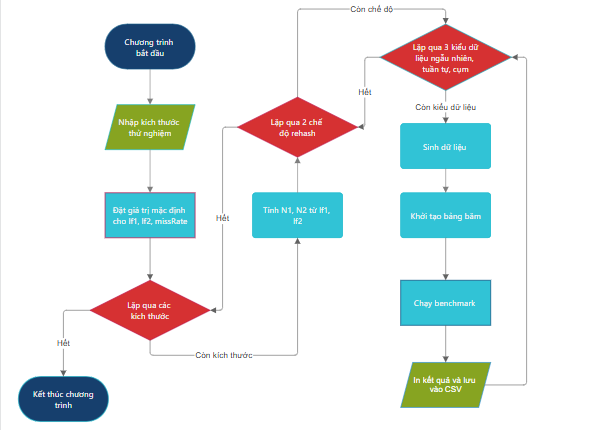
\includegraphics[width=1.0\textwidth]{fc.png}
    \caption{Sơ đồ quá trình thực hiện chương trình}
    \label{fig:flowchart}
\end{figure}
\section*{3.1. Thiết kế hệ thống thực nghiệm}
\addcontentsline{toc}{section}{{3.1. Thiết kế hệ thống thực nghiệm}}
\subsection*{3.1.1. Kiến trúc tổng thể}
\noindent \indent Hệ thống thực nghiệm được thiết kế theo mô hình modular với các thành phần chính:

- Lớp \texttt{Entry}: Biểu diễn phần tử trong bảng băm với các thuộc tính \texttt{key}, \texttt{value} và \texttt{state}.

- Lớp \texttt{HashTable}: Cài đặt cấu trúc dữ liệu bảng băm tổng quát.

- \texttt{enum SlotState}: Định nghĩa trạng thái các ô trong bảng (\texttt{EMPTY}, \texttt{OCCUPIED}, \texttt{DELETED}).

- \texttt{enum Probing}: Định nghĩa các phương pháp giải quyết xung đột.

- Lớp \texttt{Stats}: Thu thập và lưu trữ thống kê hiệu suất.

\subsection*{3.1.2. Cài đặt cấu trúc dữ liệu}

\subsubsection*{3.1.2.1. Cấu trúc \texttt{Entry}}
\begin{lstlisting}[style=numbered]
Define template structure Entry with two generic types K (key) and V (value):
    - Declare a key of type K with default value {}
    - Declare a value of type V with default value {}
    - Declare a state of type SlotState, initialized to EMPTY
\end{lstlisting}

\subsubsection*{3.1.2.2. Lớp \texttt{HashTable}}

\noindent \indent Lớp \texttt{HashTable} được thiết kế với các tham số:

- `\texttt{sz}`: Kích thước bảng băm (số nguyên tố)

- `\texttt{used}`: Số phần tử đang sử dụng

- `\texttt{type}`: Loại phương pháp dò tìm

- `\texttt{allowRehash}`: Cho phép tái cấu trúc bảng

- `\texttt{prime}`: Số nguyên tố phụ cho double hashing

\section*{3.2. Cài đặt các phương pháp giải quyết xung đột}
\addcontentsline{toc}{section}{{3.2. Cài đặt các phương pháp giải quyết xung đột}}

\subsection*{3.2.1. Linear Probing}
\begin{lstlisting}[style=numbered]
Case for Probing::LINEAR:
    Set res to base + step, where step is cast to a long long type to ensure correct type handling.
    Break out of the switch statement.
\end{lstlisting}
Phương pháp này dò tìm tuần tự từ vị trí xung đột với bước nhảy cố định là 1.

\subsection*{3.2.2. Quadratic Probing}  
\begin{lstlisting}[style=numbered]
Case for Probing::QUADRATIC:
    Set res to base + step squared (step * step), with step being cast to a long long type to ensure correct type handling.
    Break out of the switch statement.
\end{lstlisting}
Sử dụng hàm bậc hai để tính toán vị trí tiếp theo, giúp giảm primary clustering.

\subsection*{3.2.3. Double Hashing}
\begin{lstlisting}[style=numbered]
Default case:
    Set res to base + step * (prime - (key % prime)), where:
        - step is the current step count
        - prime is a prime number used for double hashing
        - key mod prime is the result of the keys hash modulo the prime number
    The calculation adjusts the probe step to reduce collisions by using a secondary hash function.
    Break out of the switch statement.
\end{lstlisting}
Áp dụng hai hàm băm:

- $h_1(k) = k mod m$: Xác định vị trí ban đầu

- $h_2(k) = R - (k mod R)$: Xác định bước nhảy ($R$ là số nguyên tố nhỏ hơn $m$)

\section*{3.3. Thiết kế thực nghiệm}
\addcontentsline{toc}{section}{{3.3. Thiết kế thực nghiệm}}

\subsection*{3.3.1. Các tham số thực nghiệm}

\subsubsection*{3.3.1.1. Hệ số tải (Load Factor)}

\noindent \indent - \texttt{LF1 = 0.5}: Hệ số tải thấp, đảm bảo hiệu suất tốt

- \texttt{LF2 = 0.9}: Hệ số tải cao, kiểm tra hiệu suất trong điều kiện khắc nghiệt

\subsubsection*{3.3.1.2. Kích thước dữ liệu}

\noindent \indent - Thực nghiệm với các kích thước khác nhau: 1000, 5000, 10000, 15000, 20000, 25000, 30000, 35000, 40000 phần tử

\subsubsection*{3.3.1.3. Tái cấu trúc bảng (Rehashing)}

\noindent \indent - Có \texttt{rehash}: Tự động tăng kích thước khi \texttt{load factor > 0.7}

- Không \texttt{rehash}: Kích thước cố định trong suốt quá trình

\subsection*{3.3.2. Mô hình dữ liệu thử nghiệm}

\subsection*{3.3.2.1. Random Pattern}
\begin{lstlisting}[style=numbered]
Function randomKV(M, keyLim):
    Create uniform integer distribution dk for key range [1, keyLim]
    Create uniform integer distribution dv for value range [1, 1000000]

    Create an empty unordered set called used
    Create an empty list called res

    While the size of res is less than M:
        Randomly generate a key k using dk(helper::rng())
        
        If key k has already been used (i.e., it is in used):
            Continue to the next iteration (skip this key)

        Add key k to used

        Randomly generate a value using dv(helper::rng())

        Add the pair (key k, value) to the list res

    Return res
\end{lstlisting}
Sinh dữ liệu ngẫu nhiên với phân phối đều.

\subsubsection*{3.3.2.2. Sequential Pattern}
\begin{lstlisting}[style=numbered]
Function sequentialKV(M):
    Create uniform integer distribution dv for value range [1, 1000000]

    Create an empty list called res
    Reserve memory for M elements in res

    For i from 1 to M:
        Randomly generate a value using dv(helper::rng())
        Add the pair (i, value) to the list res

    Return res
\end{lstlisting}
Dữ liệu tuần tự, mô phỏng worst-case cho linear probing.

\subsubsection*{3.3.2.3. Clustered Pattern}
\begin{lstlisting}[style=numbered]
Function clusteredKV(M, keyLim):
    Create uniform integer distribution dv for value range [1, 1000000]

    Set clusters = 5
    Set per = M / clusters

    Create an empty list called res
    Set base = 1

    For c from 0 to clusters - 1:
        For i from 0 to per and if the size of res is less than M:
            Randomly generate a value using dv(helper::rng())
            Add the pair (base + i, value) to the list res
        Increment base by keyLim / clusters

    Return res
\end{lstlisting}
Dữ liệu phân cụm, mô phỏng tình huống thực tế.

\subsection*{3.3.3. Các phép đo hiệu suất}

\subsubsection*{3.3.3.1. Thời gian thực thi}
\begin{lstlisting}[style=numbered]
    Get current time t1 using chrono::high_resolution_clock::now()

    Get current time t2 using chrono::high_resolution_clock::now()
    
    Calculate elapsed time in microseconds:
    Set time = duration between t1 and t2 converted to microseconds using chrono::duration_cast<chrono::microseconds>(t2 - t1).count()

    Return time
\end{lstlisting}

\noindent \indent Số lần dò tìm \textbf{(Probing Statistics)}

- Trung bình số \texttt{probe/insert}: `\texttt{stats.insProbe / stats.nIns}`

- Trung bình số \texttt{probe/search hit}: `\texttt{probeHit / hitCount}`

- Trung bình số \texttt{probe/search miss}: `\texttt{probeMiss / missCount}`

\subsubsection*{3.3.3.2. Thống kê clustering}
\begin{lstlisting}[style=numbered]
Function maxCluster():
    Initialize cur = 0, mx = 0
    
    For each element e in table:
        If e.state is OCCUPIED:
            Increment cur by 1
            Set mx to the maximum of mx and cur
        Else:
            Reset cur to 0

    Return mx (maximum cluster length)

Function avgCluster():
    Initialize cur = 0, tot = 0, cnt = 0
    
    For each element e in table:
        If e.state is OCCUPIED:
            Increment cur by 1
        Else:
            If cur is greater than 0:
                Add cur to tot
                Increment cnt by 1
                Reset cur to 0

    If cur is greater than 0:
        Add cur to tot
        Increment cnt by 1
    
    Return the average cluster length (tot / cnt) if cnt is greater than 0, otherwise return 0.0
\end{lstlisting}

\section*{3.4. Quy trình thực nghiệm}
\addcontentsline{toc}{section}{{3.4. Quy trình thực nghiệm}}

\subsection*{3.4.1. Thiết lập môi trường}
\begin{lstlisting}[style=numbered]
Create a hash table dh1 with size N1, using DOUBLE probing, and rehash allowed
Create a hash table lh1 with size N1, using LINEAR probing, and rehash allowed
Create a hash table qh1 with size N1, using QUADRATIC probing, and rehash allowed
\end{lstlisting}

\subsection*{3.4.2. Quy trình benchmark}
\begin{lstlisting}[style=numbered]
Function test(table, kv, hitIdx, missKeys, delIdx):
    Set RUN = 2

    Get current time t1 using chrono::high_resolution_clock::now()
    For each key-value pair kvp in kv:
        Insert kvp.first and kvp.second into table
    Get current time t2 using chrono::high_resolution_clock::now()

    For each index in hitIdx:
        Store the current search probe count in before
        Search for kv[hitIdx].first in table
        Add the difference between the current search probe count and before to probeHit

    For each key in missKeys:
        Store the current search probe count in before
        Search for key in table
        Add the difference between the current search probe count and before to probeMiss

    For each index in delIdx:
        Erase kv[delIdx].first from table

    For each index in delIdx:
        Store the current insert probe count in before
        Insert kv[delIdx].first back into table with a new random value
        Add the difference between the current insert probe count and before to probeInsDel

    Return result
\end{lstlisting}

\subsection*{3.4.3. Lưu trữ kết quả}
\begin{lstlisting}[style=numbered]
Function writeSummaryCSV(pattern, rehashMode, M, lf1, lf2, dh1, dh2, lh1, lh2, qh1, qh2):
    Open the file time.csv in append mode
    Write the following data to the CSV file:
        - pattern
        - rehashMode
        - M
        - dh1.insTime (insert time for dh1)
        - lh1.insTime (insert time for lh1)
        - qh1.insTime (insert time for qh1)
    Close the file
\end{lstlisting}

\section*{3.5. Công cụ phân tích và trực quan hóa}
\addcontentsline{toc}{section}{{3.5. Công cụ phân tích và trực quan hóa}}

\subsection*{3.5.1. Bảng so sánh hiệu suất}
\begin{lstlisting}[style=numbered]
Function summary(lf1, lf2, dh1, ...):
    Print header TABLE OF PERFORMANCE COMPARISON (us)

    Print the following data with proper formatting:
        - [Insert Time] LF1, dh1.insTime, lh1.insTime, qh1.insTime
        Continue printing other metrics for dh1, lh1, qh1, dh2, lh2, qh2
    
    Print other relevant metrics like search time, delete time, etc.
    Print the rest of the comparison table
\end{lstlisting}

\subsection*{3.5.2. Thống kê clustering}
\begin{lstlisting}[style=numbered]
Function printCluster(dh, lh, qh, label):
    Print header CLUSTER LENGTH STATISTICS - followed by the label

    Print the following data with proper formatting:
        - [Max cluster length]:, dh.maxCluster, lh.maxCluster, qh.maxCluster
    ....
\end{lstlisting}

\section*{3.6. Tự động hóa thực nghiệm}
\addcontentsline{toc}{section}{{3.6. Tự động hóa thực nghiệm}}

\subsection*{3.6.1. Vòng lặp thực nghiệm chính}
\begin{lstlisting}[style=numbered]
For each M in tests:
    For rehash from 0 to 1:
        For type from 1 to 3:
            Generate data kv based on the pattern (e.g., random, sequential, or clustered)
            
            Create a hash table dh1 with DOUBLE probing
            Create a hash table lh1 with LINEAR probing
            Create a hash table qh1 with QUADRATIC probing
            
            Run test for dh1, storing result in r1
            Run test for lh1, storing result in r2
            Run test for qh1, storing result in r3
            
            Call writeSummaryCSV to save the results, passing pattern, rehash, M, lf1, lf2, r1, r2, and r3
\end{lstlisting}

\subsection*{3.6.2. Xuất kết quả}
\noindent \indent Hệ thống tự động xuất kết quả ra hai file:

- \texttt{time.csv}: Thời gian thực thi các phép toán

- \texttt{clusters.csv}: Thống kê về độ dài cluster

\section*{3.7. Đảm bảo tính tin cậy}
\addcontentsline{toc}{section}{{3.7. Đảm bảo tính tin cậy}}

\subsection*{3.7.1. Lặp lại thử nghiệm}
\noindent \indent Mỗi test case được chạy 2 lần (`\texttt{const int RUN = 2}`) để giảm thiểu sai số do biến động hệ thống.

\subsection*{3.7.2. Kiểm soát biến số}

\noindent \indent - Sử dụng `\texttt{mt19937}` với seed cố định để có thể tái tạo kết quả

- Kiểm soát chặt chẽ các tham số: kích thước bảng, hệ số tải, loại dữ liệu

\subsection*{3.7.3. Đo lường chính xác}

\noindent \indent - Sử dụng `\texttt{chrono::high\_resolution\_clock}` cho độ chính xác cao

- Đo riêng biệt từng loại phép toán (insert, search, delete)







\newpage
\chapter*{\centering{\MakeUppercase{Chương IV. Phân tích và đánh giá kết quả}}}
\addcontentsline{toc}{chapter}{\textcolor{fitblue}{\MakeUppercase{Chương IV. Phân tích và đánh giá kết quả}}}
\section*{4.1. Đầu vào ngẫu nhiên}
\addcontentsline{toc}{section}{{4.1. Đầu vào ngẫu nhiên}}
\subsection*{4.1.1. Cluster trung bình}
\begin{figure}[!ht]
    \centering
    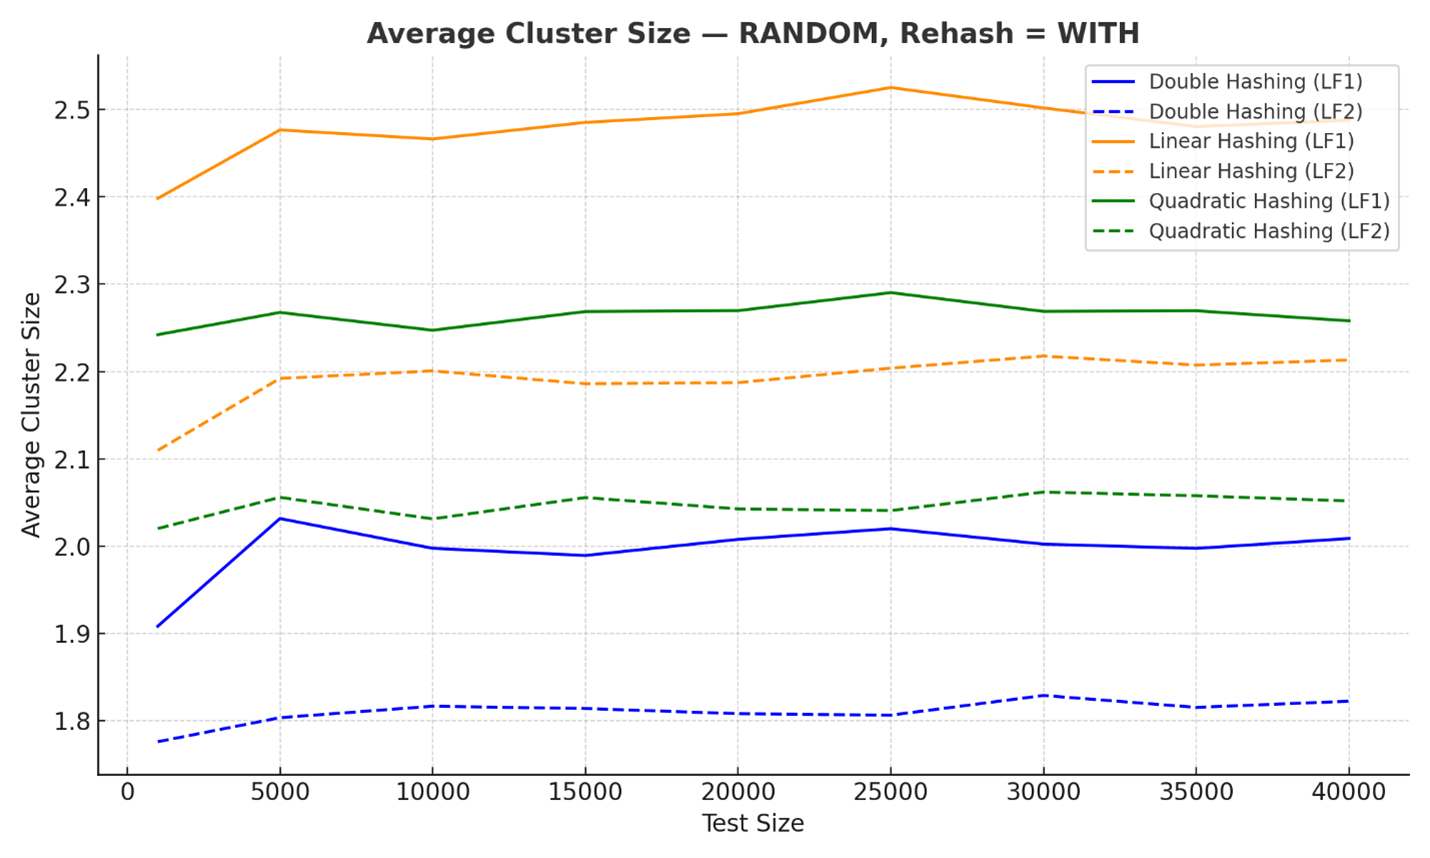
\includegraphics[width=0.8\textwidth]{ran_avr_clus.png}
    \caption{Đồ thị cluster trung bình theo số lượng phần tử của bảng băm có rehash với kiểu đầu vào ngẫu nhiên}
    \label{fig:flowchart}
\end{figure}
    -	Double Hashing có số cluster trung bình so với Linear hashing và Quadaric Hashing ở mọi mức tải. Trong tải trung bình (LF1), số cluster trung bình của DH dao động quanh 2, thấp hơn đáng kể so với LH (trên 2.4) và QH (\textasciitilde 2.26). Trong điều kiện tải cao (LF2), sự chênh lệch càng rõ: LH thường vượt mốc 2.2, còn DH ổn định quanh mức 1.8.
    
-	Số cluster tối đa (Max) của DH cũng thấp hơn nhiều, chỉ từ 8–18 trong hầu hết thử nghiệm, trong khi LH thường vượt 30, thậm chí lên đến 38. Điều này phản ánh đặc trưng nổi bật của Double Hashing là khả năng phân tán tốt và tránh clustering hiệu quả.
\newpage
\subsection*{4.1.2. Thời gian thực hiện các thao tác}
\begin{figure}[!ht]
    \centering
    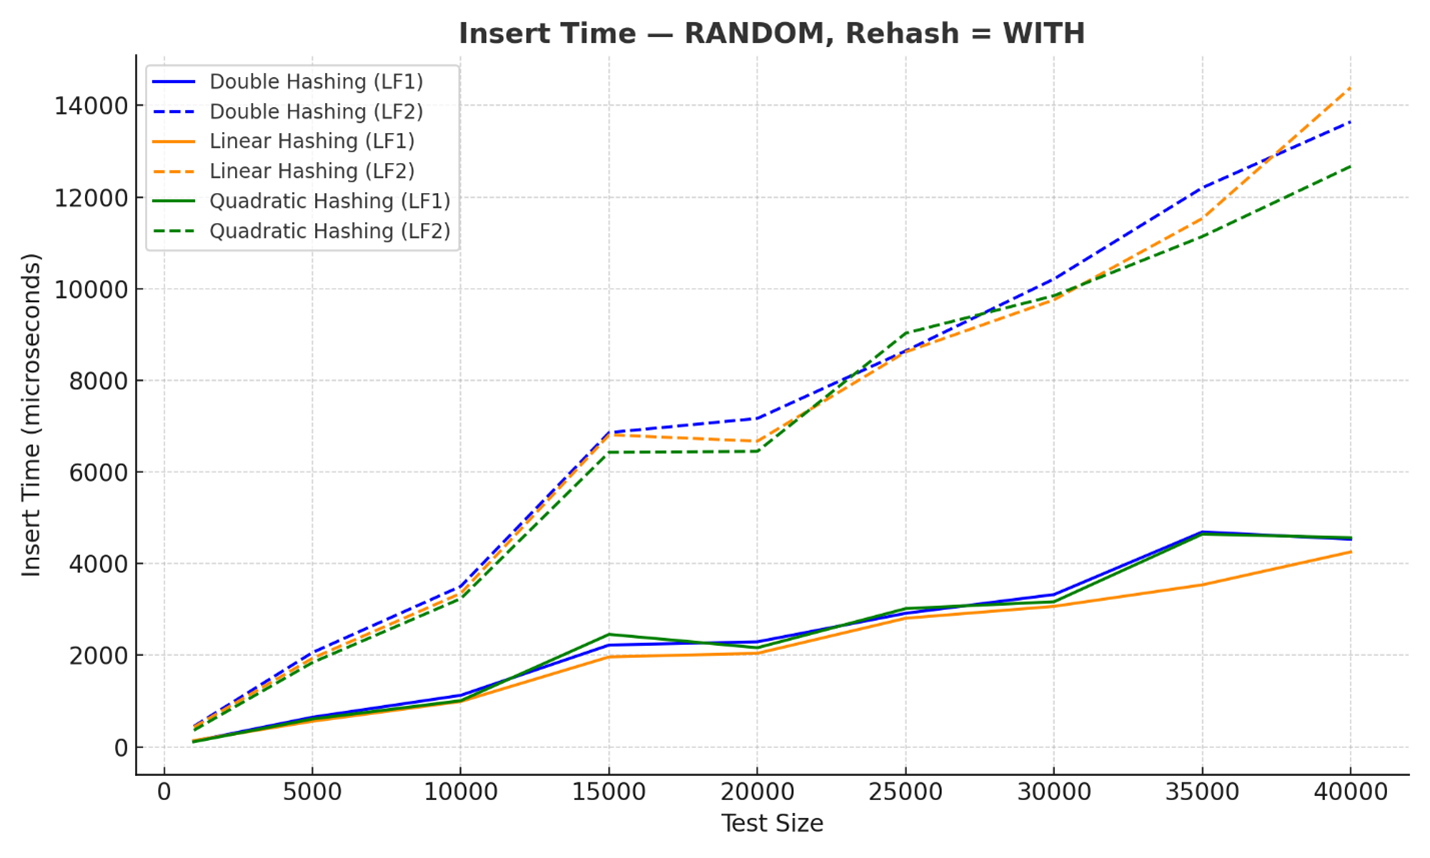
\includegraphics[width=0.8\textwidth]{ran_ser_hash.png}
    \caption{Đồ thị thời gian chèn theo số lượng phần tử của bảng băm có rehash với kiểu đầu vào ngẫu nhiên}
    \label{fig:flowchart}
\end{figure}

\begin{figure}[!ht]
    \centering
    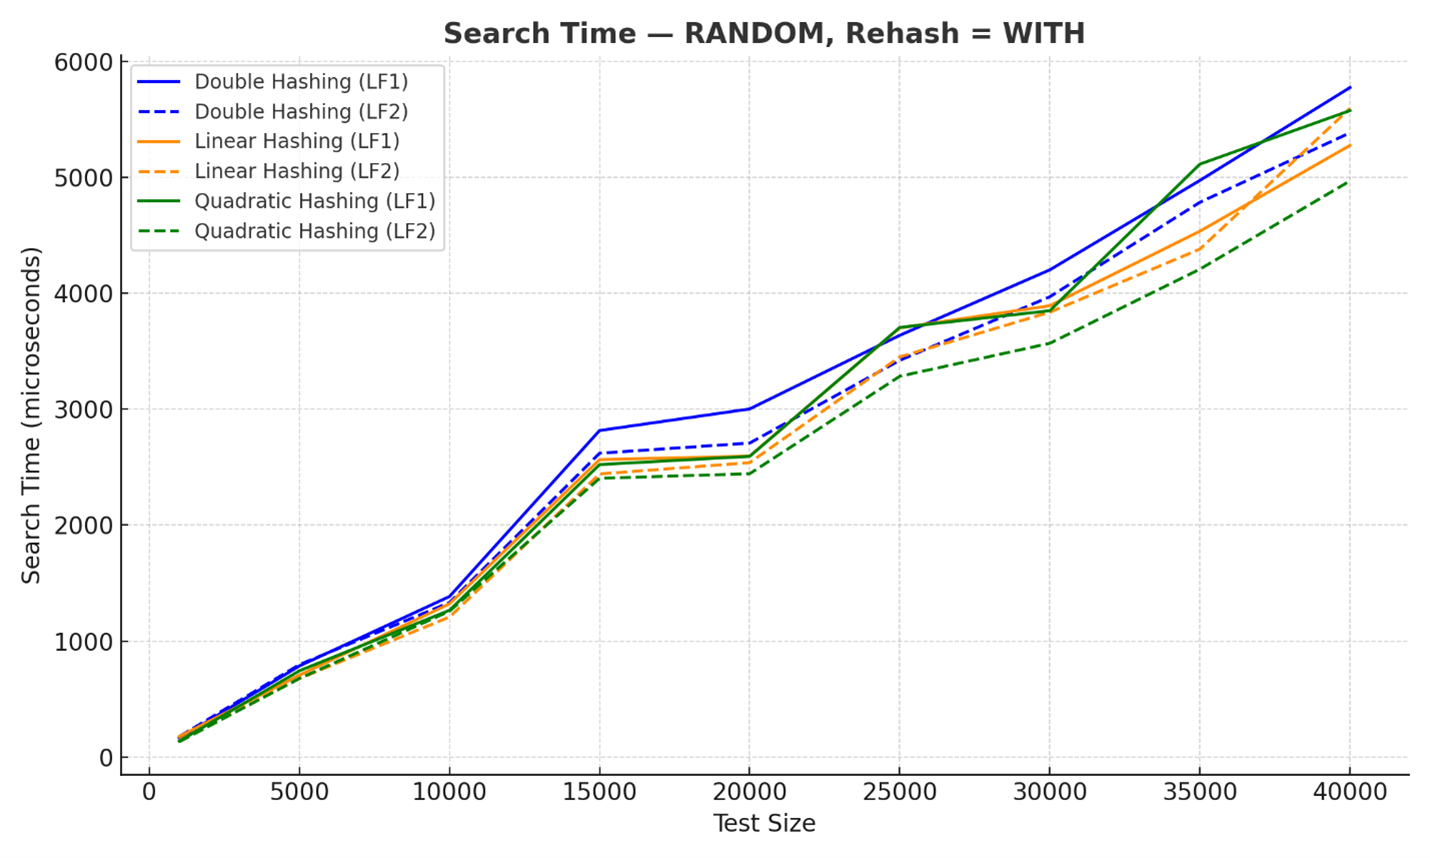
\includegraphics[width=0.8\textwidth]{ran_search_hash.png}
    \caption{Đồ thị thời gian tìm theo số lượng phần tử của bảng băm có rehash với kiểu đầu vào ngẫu nhiên}
    \label{fig:flowchart}
\end{figure}

\begin{figure}[!ht]
    \centering
    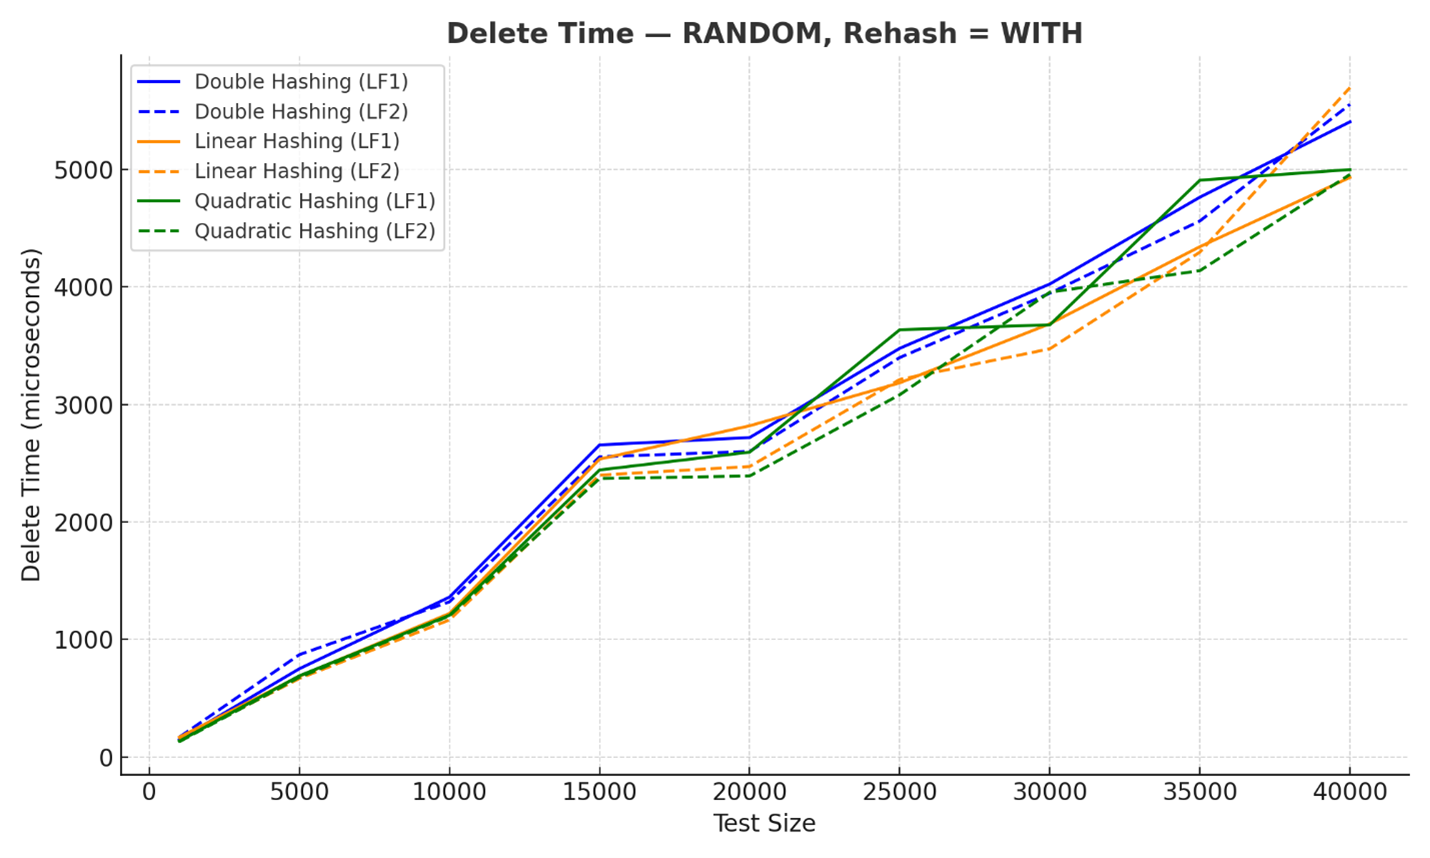
\includegraphics[width=0.8\textwidth]{ran_del_hash.png}
    \caption{Đồ thị thời gian xóa theo số lượng phần tử của bảng băm có rehash với kiểu đầu vào ngẫu nhiên}
    \label{fig:flowchart}
\end{figure}
\noindent \indent-	Ở bảng nhỏ và tải nhẹ, ba kỹ thuật có thời gian thao tác gần nhau. Tuy nhiên, khi kích thước và tải tăng lên, sự khác biệt rõ rệt xuất hiện.

-	Insert: Double Hashing duy trì thời gian tốt ở mức trung bình, dù có xu hướng tăng hơn QH trong bảng rất lớn, do chi phí tính toán hai hàm băm. Tuy nhiên, sự tăng này vẫn trong giới hạn có thể chấp nhận được.

-	Search: Là nơi DH thể hiện ưu thế rõ rệt. Ở bảng 50,000 phần tử với tải cao, thời gian tìm kiếm bằng LH cao gấp 2.7 lần so với DH, do LH bị ảnh hưởng nặng bởi clustering. QH cho kết quả khá tốt nhưng kém ổn định.

-	Delete: Hiệu suất delete của DH khá ổn định và tốt hơn LH trong phần lớn các trường hợp. QH có kết quả gần DH trong delete, nhưng lại thiếu nhất quán ở các kích thước khác nhau.
\subsection*{4.1.3. Hiệu năng khi không rehash}
\begin{figure}[!ht]
    \centering
    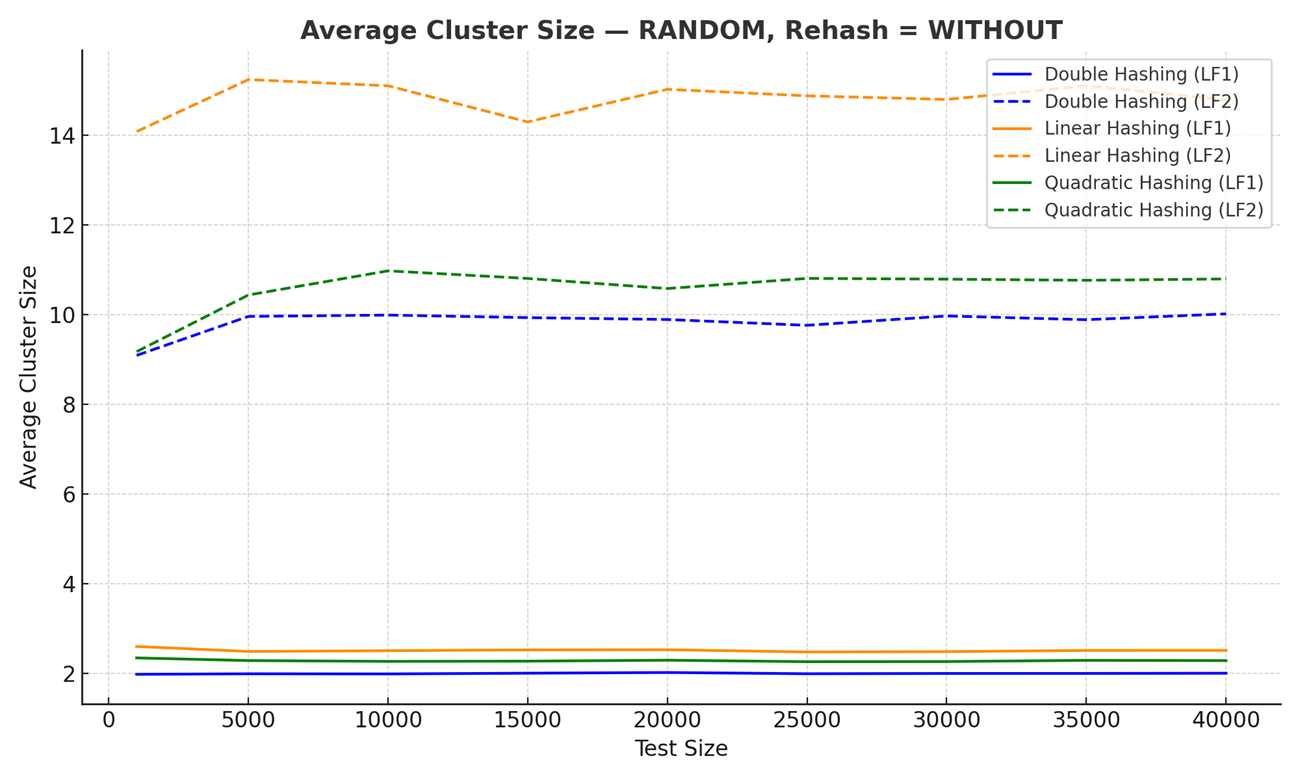
\includegraphics[width=0.8\textwidth]{ran_avr_not.png}
    \caption{Đồ thị cluster trung bình theo số lượng phần tử của bảng băm không có rehash với kiểu đầu vào ngẫu nhiên}
    \label{fig:flowchart}
\end{figure}

\begin{figure}[!ht]
    \centering
    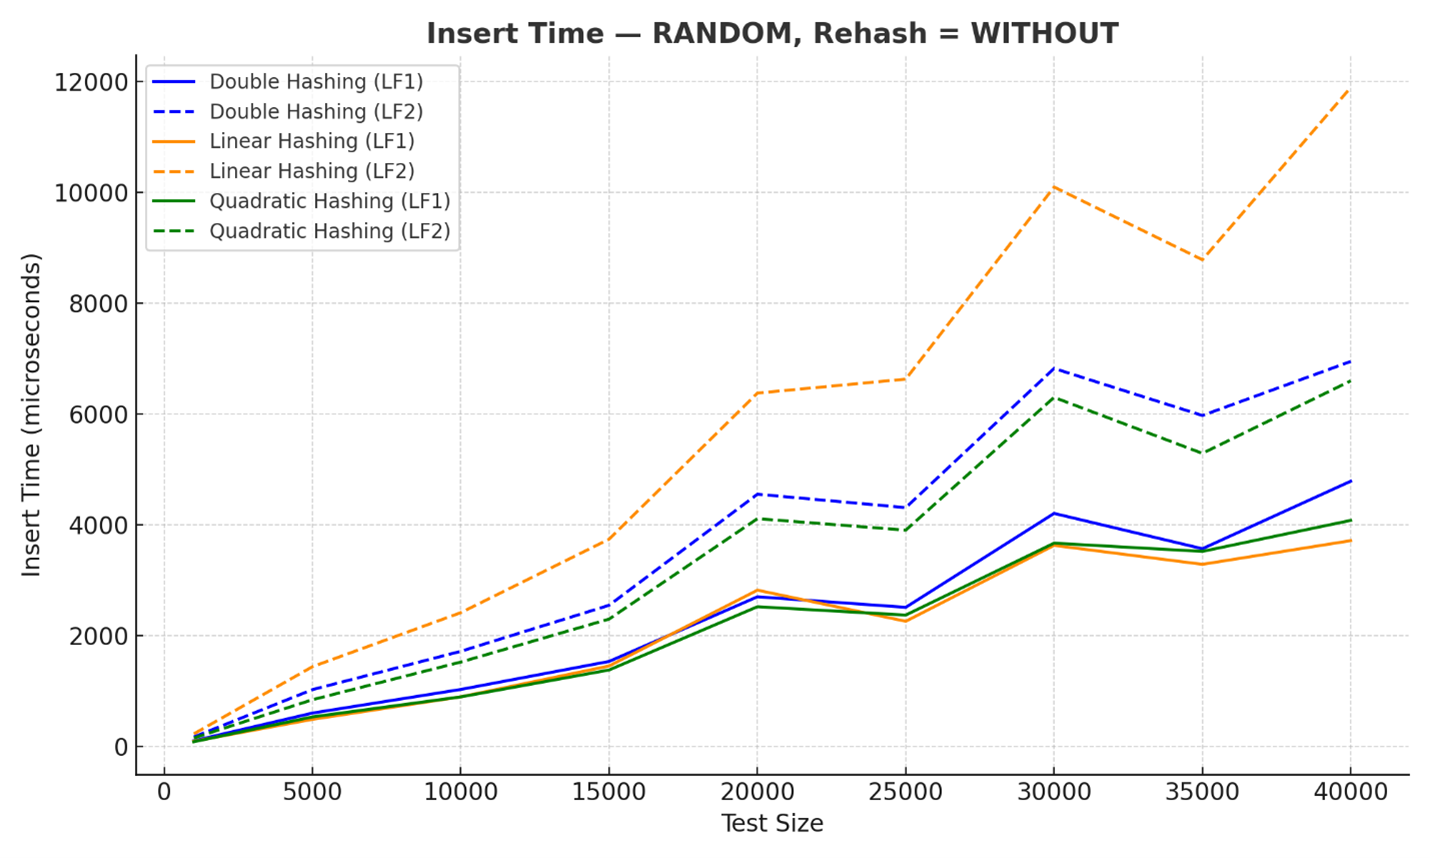
\includegraphics[width=0.8\textwidth]{ran_ser_not.png}
    \caption{Đồ thị thời gian chèn theo số lượng phần tử của bảng băm không có rehash với kiểu đầu vào ngẫu nhiên}
    \label{fig:flowchart}
\end{figure}

\begin{figure}[!ht]
    \centering
    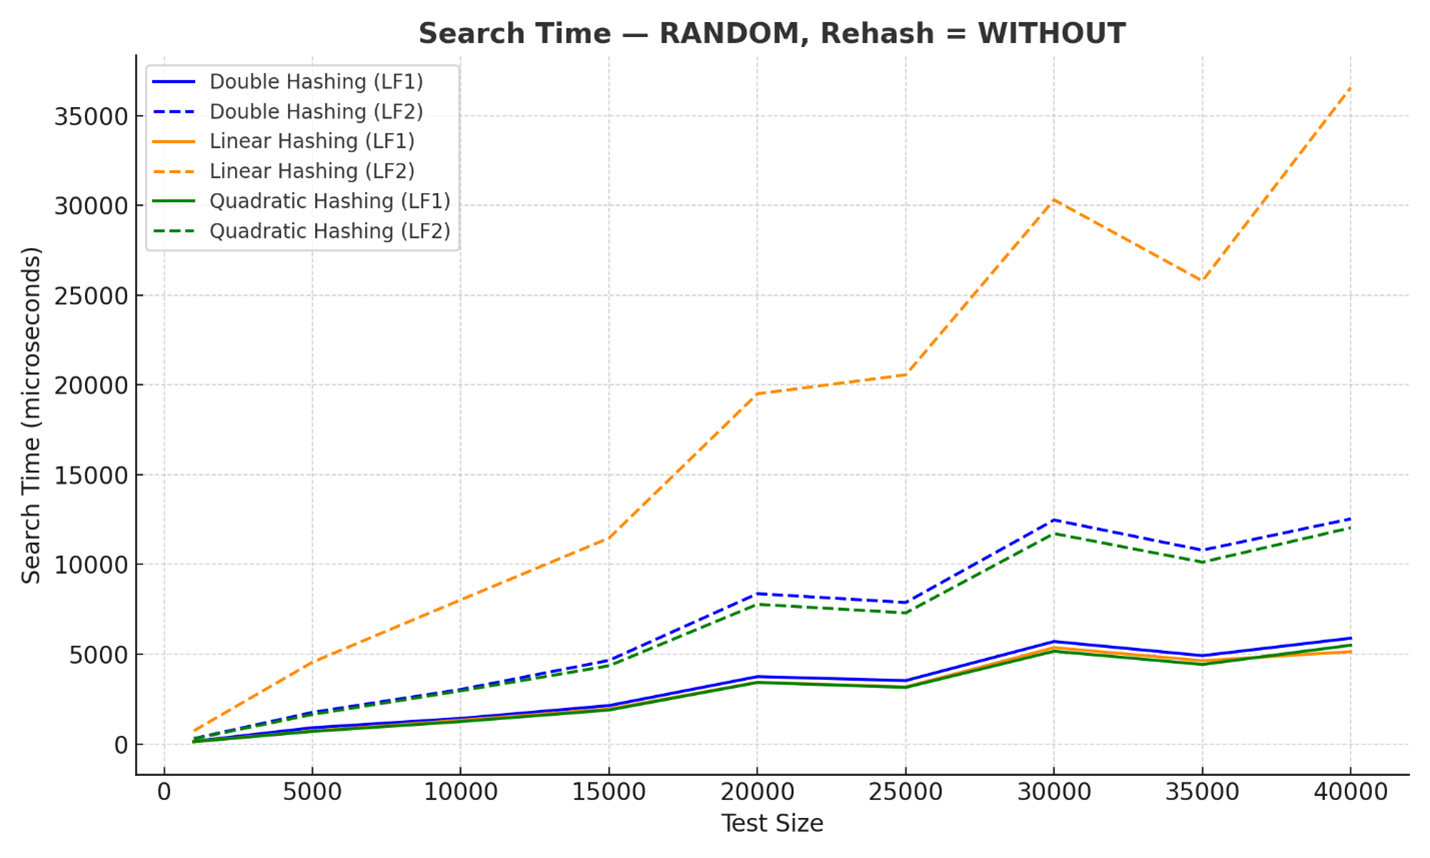
\includegraphics[width=0.8\textwidth]{ran_search_not.png}
    \caption{Đồ thị thời gian tìm theo số lượng phần tử của bảng băm không có rehash với kiểu đầu vào ngẫu nhiên}
    \label{fig:flowchart}
\end{figure}

\begin{figure}[!ht]
    \centering
    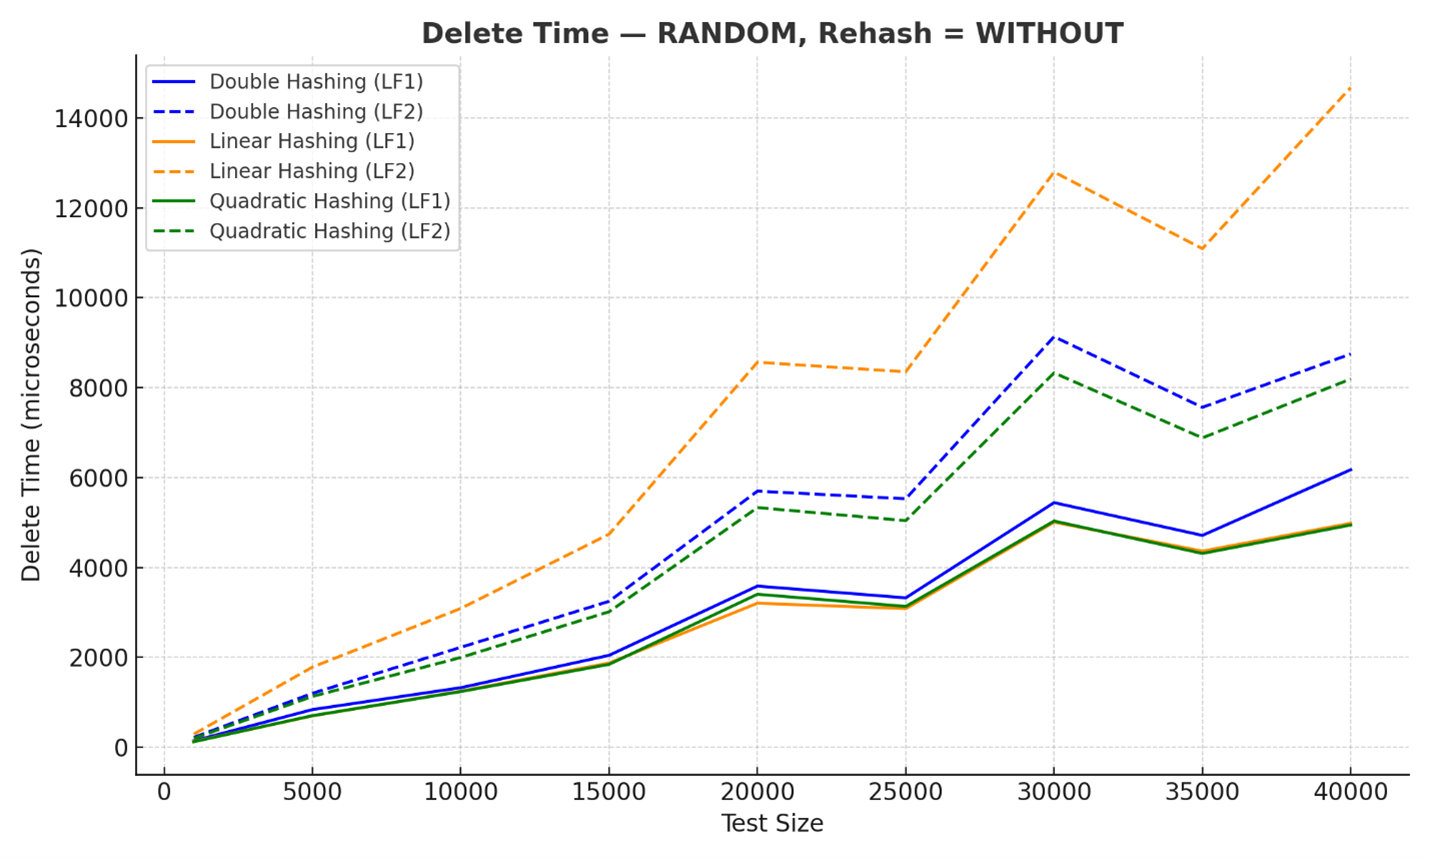
\includegraphics[width=0.8\textwidth]{ran_del_not.png}
    \caption{Đồ thị thời gian xóa theo số lượng phần tử của bảng băm không có rehash với kiểu đầu vào ngẫu nhiên}
    \label{fig:flowchart}
\end{figure}
-	Khi bảng đầy, tất cả các kỹ thuật đều có số cluster trung bình tăng mạnh. Tuy nhiên, DH tiếp tục thể hiện tính ổn định: số cluster trung bình của nó giữ ở mức \textasciitilde 10, trong khi LH tăng đến hơn 15. QH cũng bị ảnh hưởng, nhưng thấp hơn LH.

-	Trong điều kiện không rehash, các chỉ số thời gian đều tăng đột biến – đặc biệt với LH. Điều này củng cố giả thiết rằng nếu không tái cấu trúc bảng băm khi tải cao, DH là lựa chọn tối ưu nhất.
\newpage
\subsection*{4.1.4. Đánh giá tổng quan}
\noindent \indent \textbf{Double Hashing (DH):}

- Ưu điểm:

\hspace{1cm}+ Hiệu suất phân phối tránh clustering tốt nhất (cả trung bình và cực trị).

\hspace{1cm}+	Ổn định khi bảng lớn hoặc gần đầy.

\hspace{1cm}+	Tránh clustering hiệu quả.

-	Nhược điểm:	Chậm hơn một chút khi insert bảng rất lớn (do tính hai hàm băm).

	\textbf{Linear Probing (LH):}
    
-	Ưu điểm: đơn giản, nhanh ở bảng nhỏ.

-	Nhược điểm: clustering nghiêm trọng, giảm hiệu năng rõ rệt ở bảng lớn hoặc tải cao.

	\textbf{Quadratic Probing (QH):}
    
-	Ưu điểm: cân bằng giữa đơn giản và giảm clustering.
-	Nhược điểm: hiệu suất không ổn định, có thể bị kẹt trong secondary clustering.


\section*{4.2. Đầu vào tuần tự}
\addcontentsline{toc}{section}{{4.2. Đầu vào tuần tự}}
\subsection*{4.2.1. Cluster trung bình}
\begin{figure}[!ht]
    \centering
    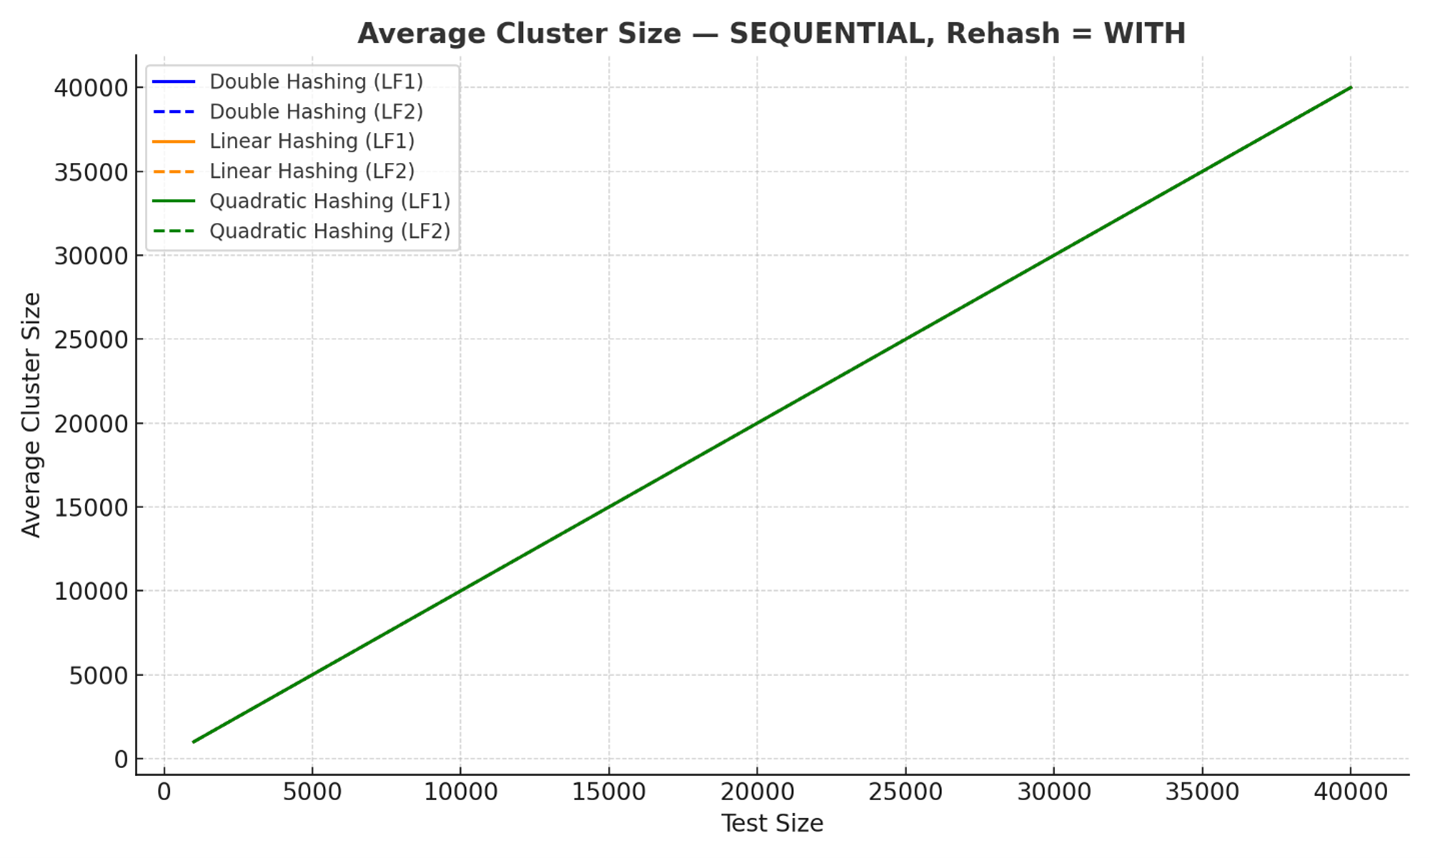
\includegraphics[width=0.8\textwidth]{seq_clus_hash.png}
    \caption{Đồ thị cluster trung bình theo số lượng phần tử của bảng băm có rehash với kiểu đầu vào tuần tự}
    \label{fig:flowchart}
\end{figure}
\noindent \indent -Double Hashing (DH) có kích thước cluster thấp nhất so với Linear Hashing (LH) và Quadratic Hashing (QH) ở cả hai mức tải.

-	Với tải trung bình (LF1), DH dao động quanh \textasciitilde 2, trong khi LH vượt 2.4 và QH xấp xỉ 2.26.

-	Với tải cao (LF2), chênh lệch rõ rệt hơn: DH giữ ổn định quanh 1.8, trong khi LH vượt 2.2.

\subsection*{4.2.2. Thời gian thực hiện các thao tác}
\begin{figure}[!ht]
    \centering
    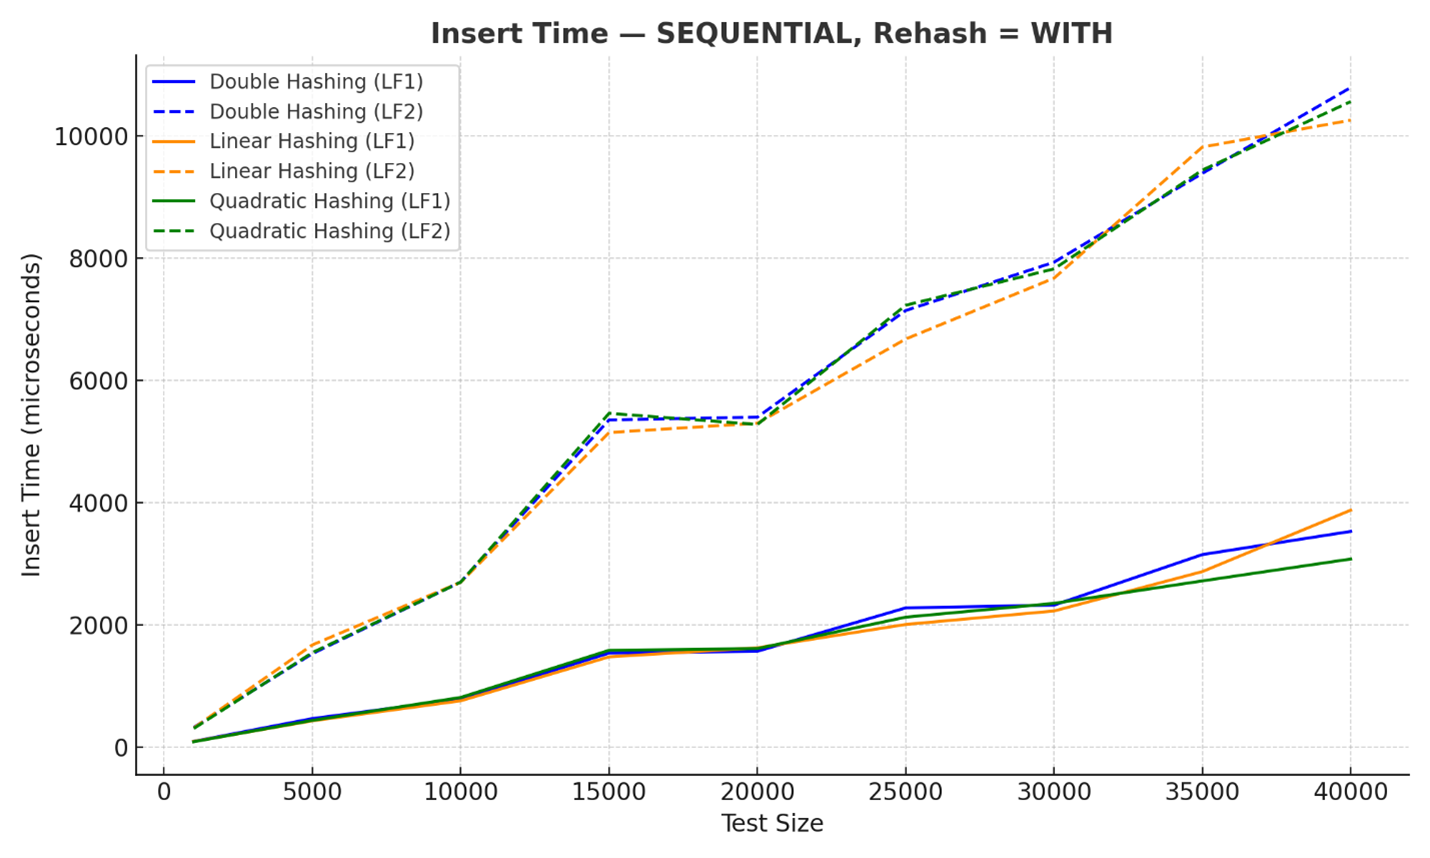
\includegraphics[width=0.8\textwidth]{seq_ins_hash.png}
    \caption{Đồ thị thời gian tìm theo số lượng phần tử của bảng băm có rehash với kiểu đầu vào tuần tự}
    \label{fig:flowchart}
\end{figure}

\begin{figure}[!ht]
    \centering
    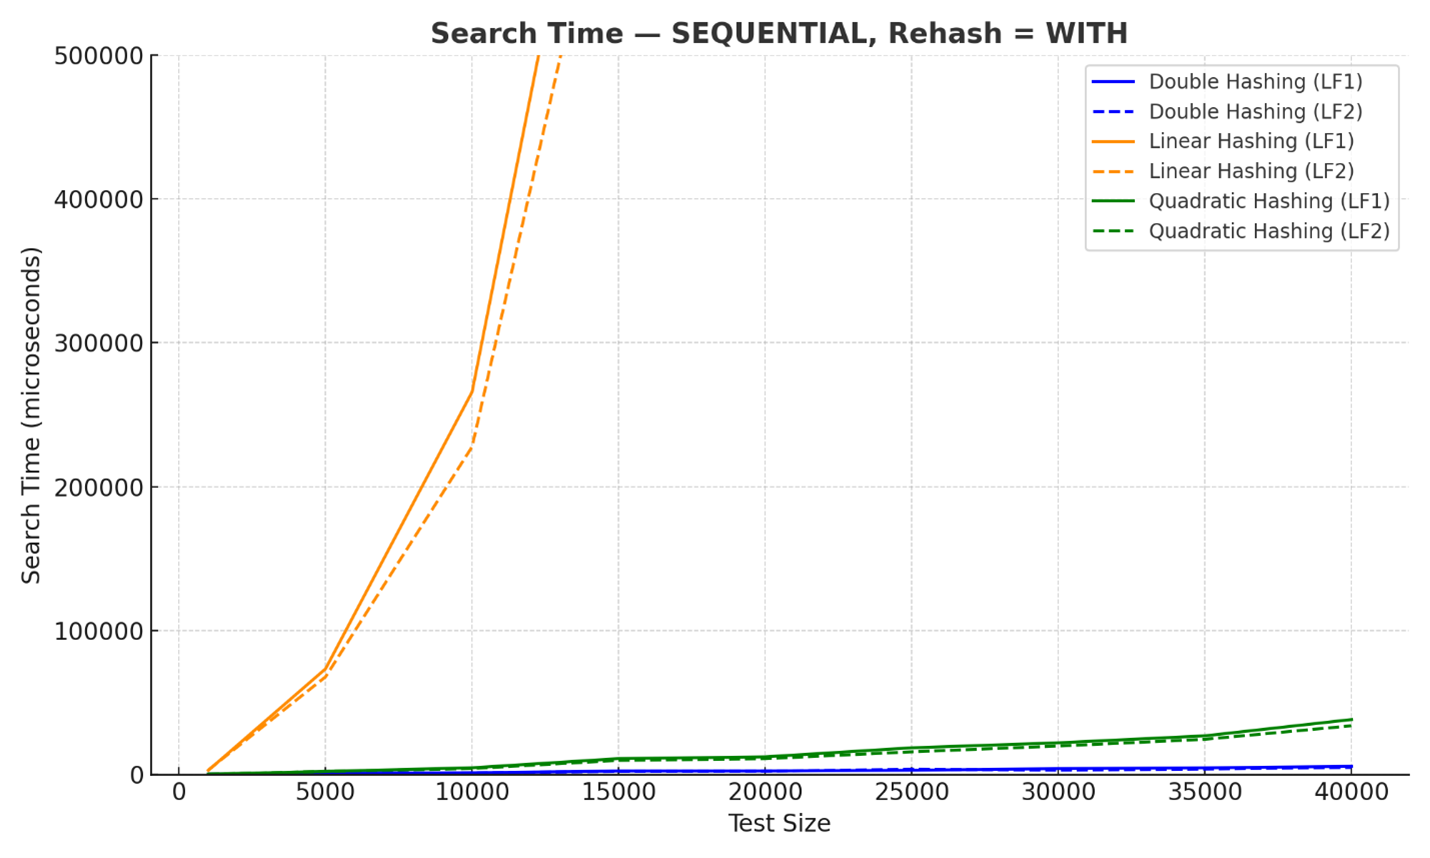
\includegraphics[width=0.8\textwidth]{seq_sear_hash.png}
    \caption{Đồ thị thời gian tìm theo số lượng phần tử của bảng băm có rehash với kiểu đầu vào tuần tự}
    \label{fig:flowchart}
\end{figure}

\begin{figure}[!ht]
    \centering
    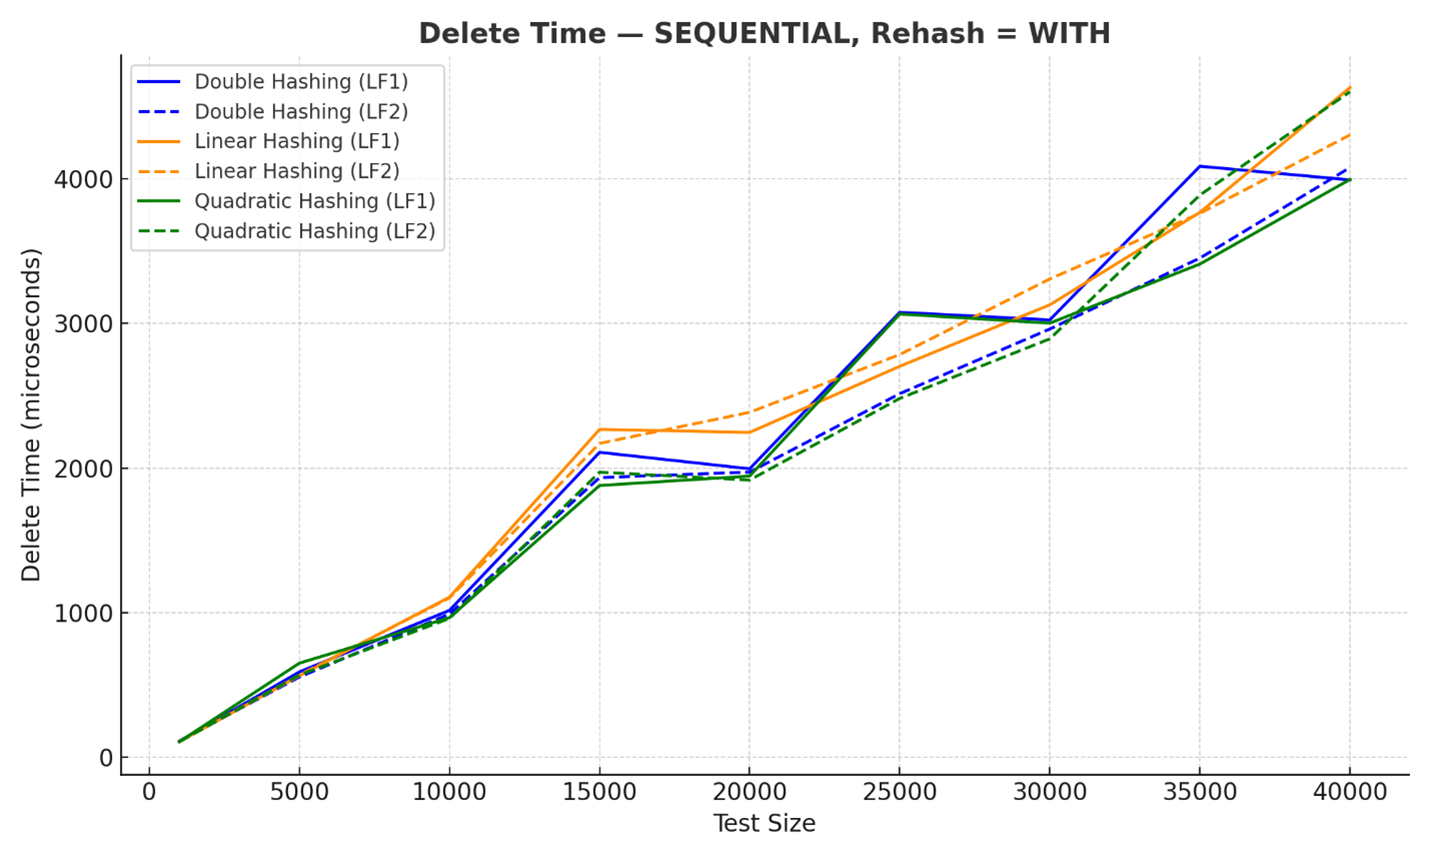
\includegraphics[width=0.8\textwidth]{seq_del_hash.png}
    \caption{Đồ thị thời gian xóa theo số lượng phần tử của bảng băm có rehash với kiểu đầu vào tuần tự}
    \label{fig:flowchart}
\end{figure}
\noindent \indent \textbf{Insert:}

-	Với bảng nhỏ và tải nhẹ, thời gian insert giữa ba kỹ thuật không chênh lệch nhiều.

-	Khi bảng lớn và tải cao, thời gian insert của DH tăng do tính hai hàm băm, nhưng vẫn trong mức chấp nhận được.

-	QH có insert nhanh hơn ở bảng rất lớn, nhưng không đáng kể so với lợi ích phân tán mà DH mang lại.

 \textbf{Search:}
 
-	DH thể hiện ưu thế vượt trội.

-	Ở bảng 50.000 phần tử, LH mất thời gian tìm kiếm gấp \textasciitilde 2.7 lần DH.

-	QH có hiệu suất tốt hơn LH nhưng kém ổn định hơn DH.

	\textbf{Delete:}
    
-	DH duy trì hiệu suất delete ổn định và nhất quán, ngay cả ở bảng lớn.

-	LH thường bị giảm hiệu năng delete do thời gian dò tìm vị trí tăng cao.

-	QH đôi khi đạt hiệu quả gần với DH, nhưng thiếu ổn định giữa các kích thước bảng khác nhau.
\newpage
\subsection*{4.2.3. Hiệu năng khi không rehash}

\begin{figure}[!ht]
    \centering
    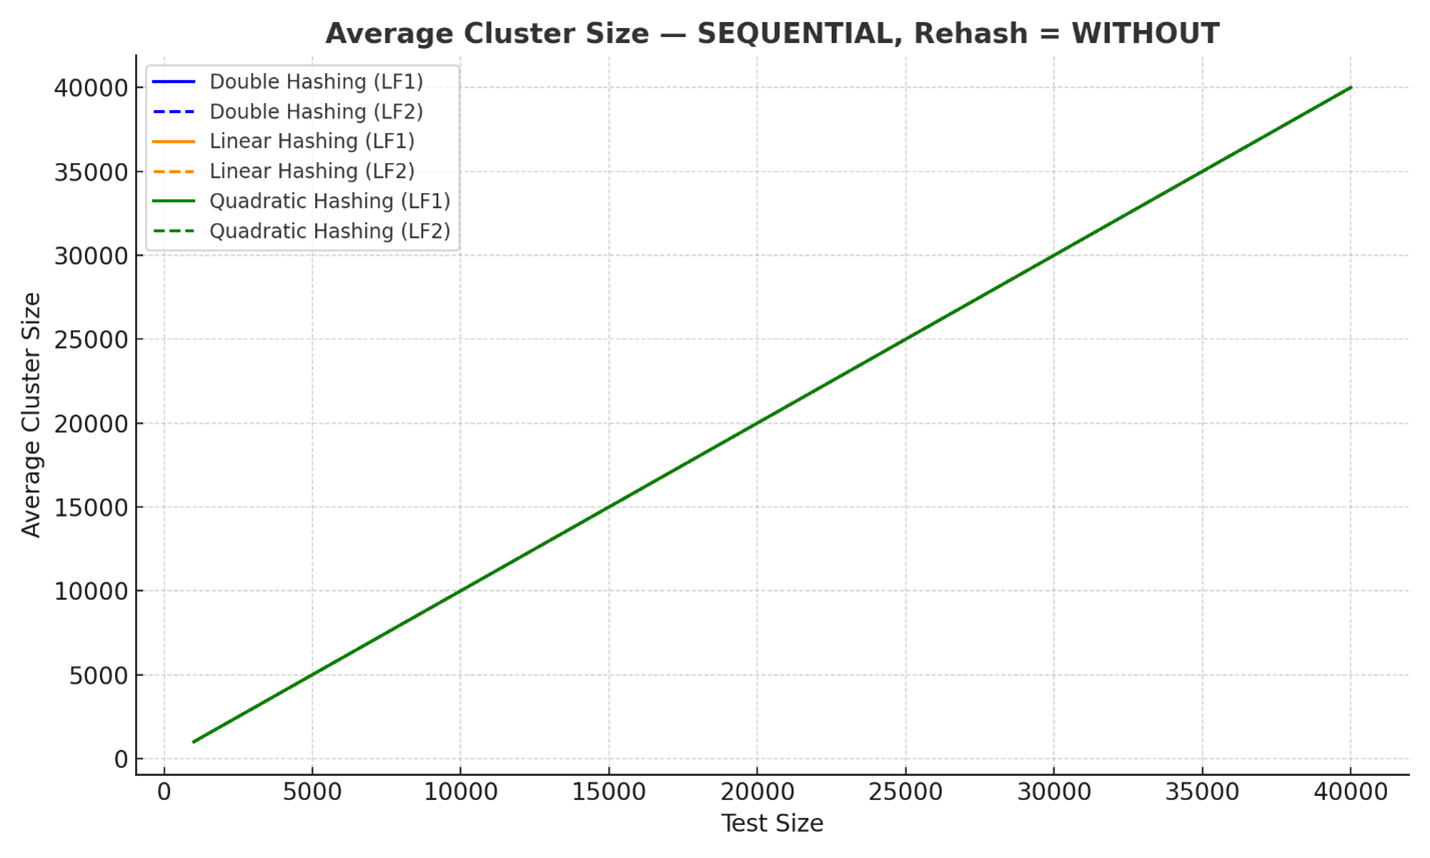
\includegraphics[width=0.8\textwidth]{seq_clus_not.png}
    \caption{Đồ thị cluster trung bình theo số lượng phần tử của bảng băm không có rehash với kiểu đầu vào tuần tự}
    \label{fig:flowchart}
\end{figure}

\begin{figure}[!ht]
    \centering
    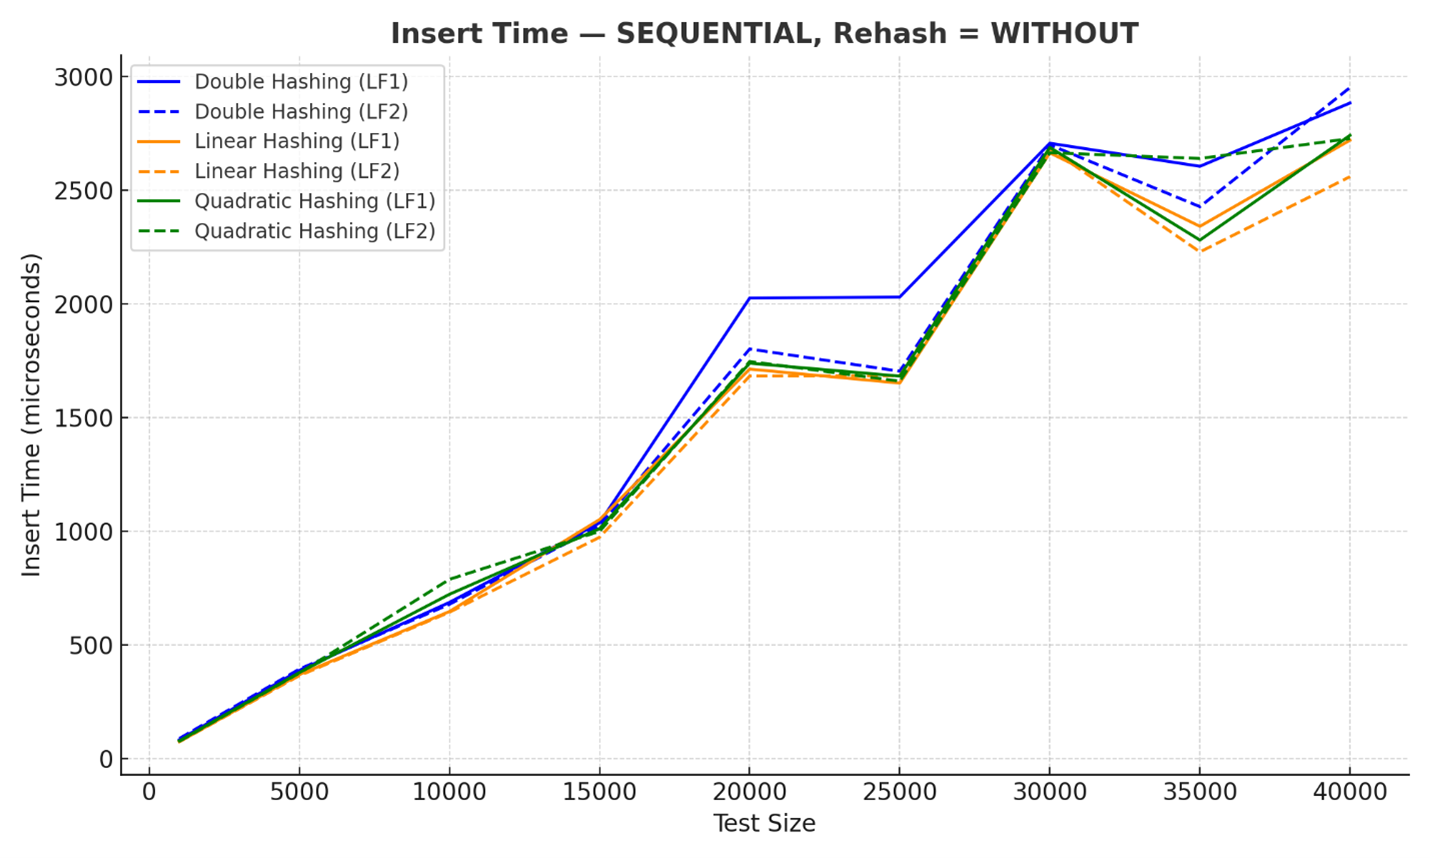
\includegraphics[width=0.8\textwidth]{seq_ins_not.png}
    \caption{Đồ thị thời gian chèn theo số lượng phần tử của bảng băm không có rehash với kiểu đầu vào tuần tự}
    \label{fig:flowchart}
\end{figure}

\begin{figure}[!ht]
    \centering
    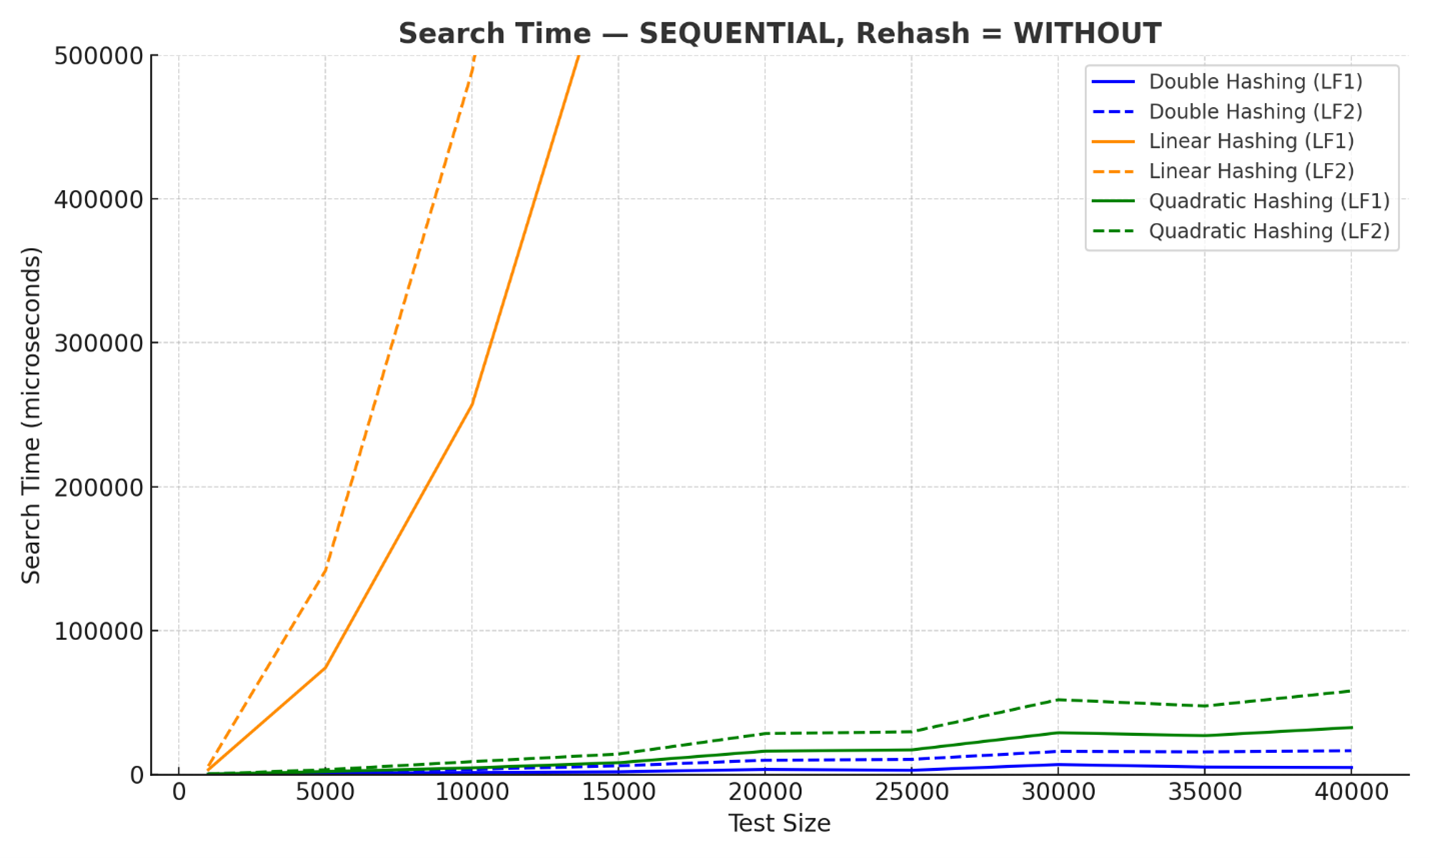
\includegraphics[width=0.8\textwidth]{seq_sear_not.png}
    \caption{Đồ thị thời gian tìm theo số lượng phần tử của bảng băm không có rehash với kiểu đầu vào tuần tự}
    \label{fig:flowchart}
\end{figure}

\begin{figure}[!ht]
    \centering
    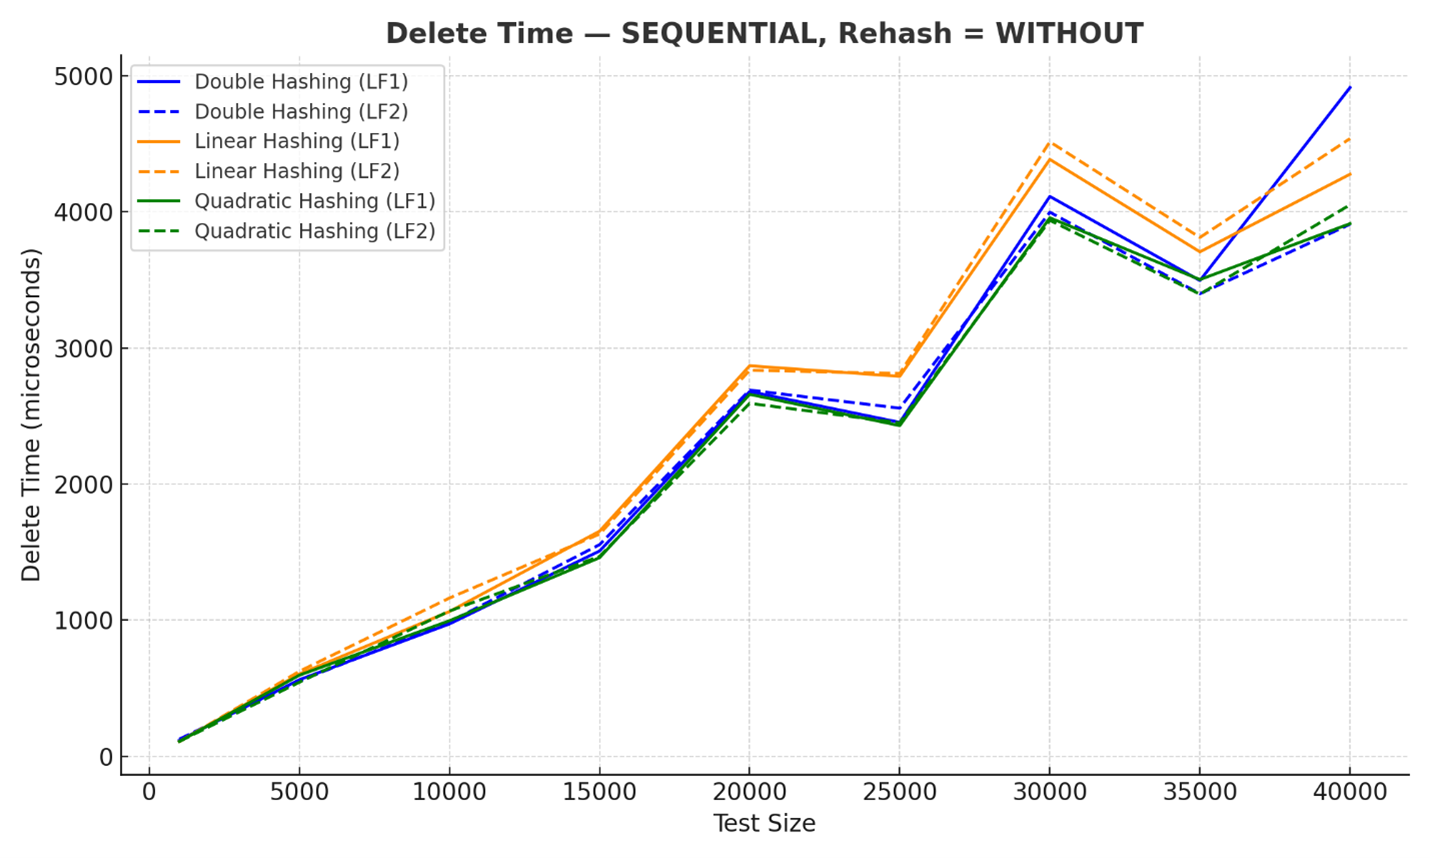
\includegraphics[width=0.8\textwidth]{seq_del_not.png}
    \caption{Đồ thị thời gian xóa theo số lượng phần tử của bảng băm không có rehash với kiểu đầu vào tuần tự}
    \label{fig:flowchart}
\end{figure}

\noindent \indent \textbf{Số cluster trung bình:}

-	Khi bảng đầy và không tái cấu trúc, mọi kỹ thuật đều bị suy giảm hiệu năng.

-	DH vẫn giữ số cluster trung bình quanh \textasciitilde 10.

-	LH tăng mạnh, vượt mốc 15 — biểu hiện rõ của primary clustering.

-	QH tăng ít hơn LH nhưng vẫn bị ảnh hưởng nặng.

\textbf{Thời gian thực tế:}

-	Tất cả thao tác (insert, search, delete) đều tăng thời gian đáng kể.

-	LH bị ảnh hưởng nặng nhất, có thời gian search tăng đến hàng triệu đơn vị.

-	DH vẫn giữ thời gian trong mức kiểm soát, dù có tăng.

\textbf{Kết luận:}

-	Trong môi trường không rehash, DH chứng minh được khả năng “sống sót” và duy trì hiệu năng.

-	LH và QH nhanh chóng mất hiệu quả do clustering nghiêm trọng.

\subsection*{4.2.4. Đánh giá tổng quan}

\noindent \indent \textbf{Double Hashing (DH):}

- Ưu điểm:

\hspace{1cm}+	Hiệu suất phân phối các khoá và tránh clustering tốt nhất (trung bình và cực trị).

\hspace{1cm}+	Ổn định ở bảng lớn, gần đầy, hoặc không rehash.

\hspace{1cm}+	Giảm clustering hiệu quả nhờ bước dò phụ độc lập.

-	Nhược điểm: Chậm hơn một chút khi insert ở bảng rất lớn (do phải tính hai hàm băm).

	\textbf{Linear Probing (LH):}


-	Ưu điểm: Thuật toán đơn giản, hiệu quả tốt khi bảng nhỏ và tải nhẹ.


-	Nhược điểm:


\hspace{1cm}+	Clustering rất nghiêm trọng, đặc biệt là khi bảng gần đầy.


\hspace{1cm}+	Hiệu suất giảm mạnh với bảng lớn hoặc dữ liệu tăng đều.


\textbf{Quadratic Probing (QH):}

-	Ưu điểm: Tránh được primary clustering, hiệu quả hơn LH trong đa số trường hợp.

-	Nhược điểm:

\hspace{1cm}+	Có thể gặp secondary clustering.

\hspace{1cm}+	Hiệu suất thiếu ổn định, phụ thuộc vào hàm băm và phân bố dữ liệu.
\section*{4.3. Đầu vào phân cụm}
\addcontentsline{toc}{section}{{4.3. Đầu vào phân cụm}}
\subsection*{4.3.1. Cluster trung bình}
\begin{figure}[!ht]
    \centering
    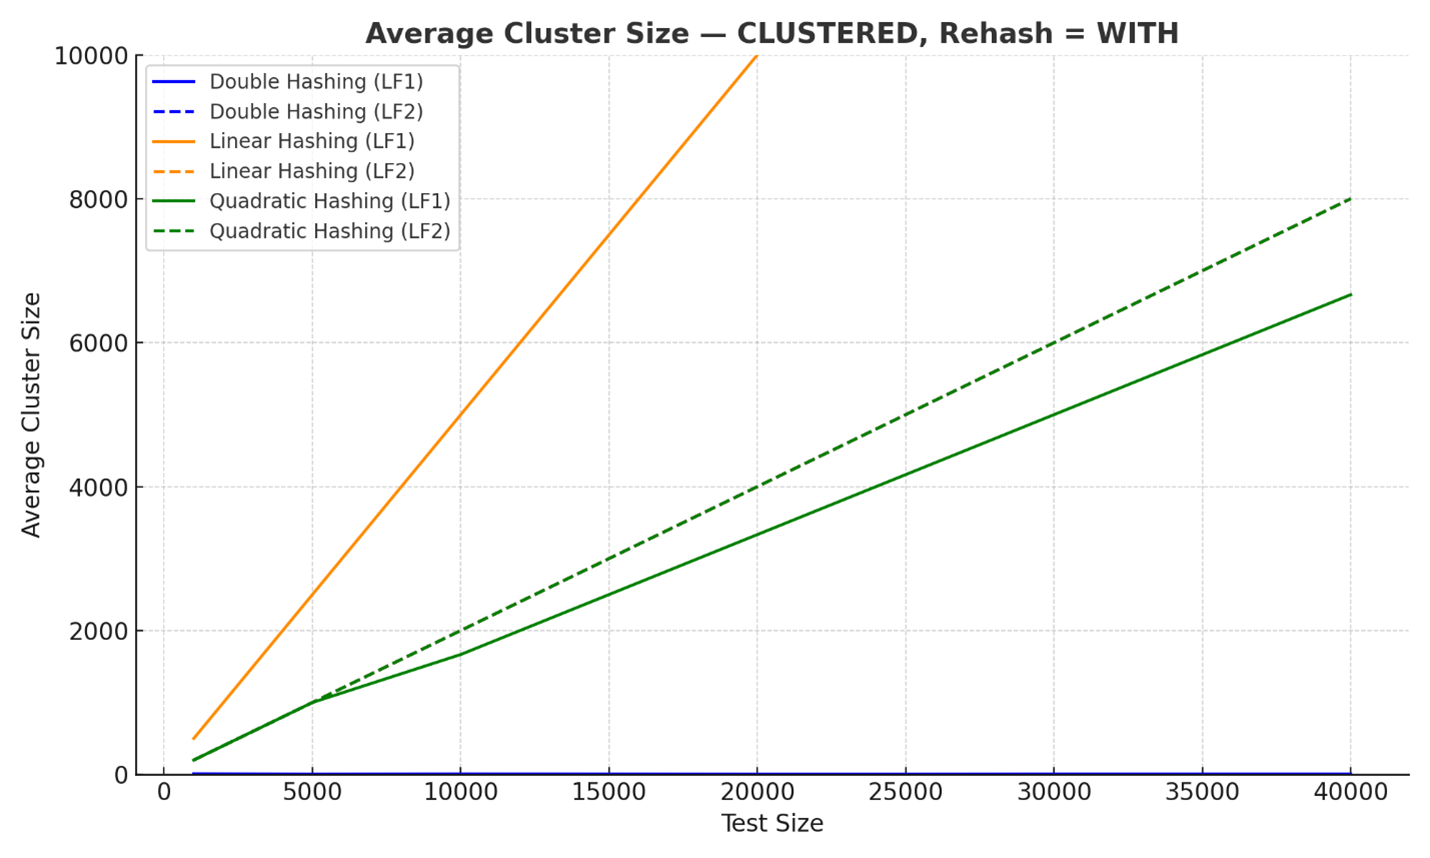
\includegraphics[width=0.8\textwidth]{clus_clus_hash.png}
    \caption{Đồ thị cluster trung bình theo số lượng phần tử của bảng băm có rehash với kiểu đầu vào phân cụm}
    \label{fig:flowchart}
\end{figure}
\noindent \indent -	Double Hashing luôn trì hiệu suất tốt nhất dao động từ 5 – 8 cluster (gần như bằng 0) trong khi đó Linear Hashing cho thấy hiệu suất tệ nhất cluster bằng ½ kích thước của bảng,Quadratic Hashing giảm thiểu được cluster tốt hơn nhiều so với Linear Hashing nhưng nó vẫn có thể gặp phải secondary clustering (phân cụm thứ cấp) khi các phần tử băm đến cùng một vị trí ban đầu sẽ theo cùng một chuỗi dò tìm.

-	Với LF2 cả ba kiểu hashing đều cho cùng 1 số lượng cluster trung bình khoảng 1/5 kích thước bảng


\subsection*{4.3.2. Thời gian thực hiện các thao tác}
\begin{figure}[!ht]
    \centering
    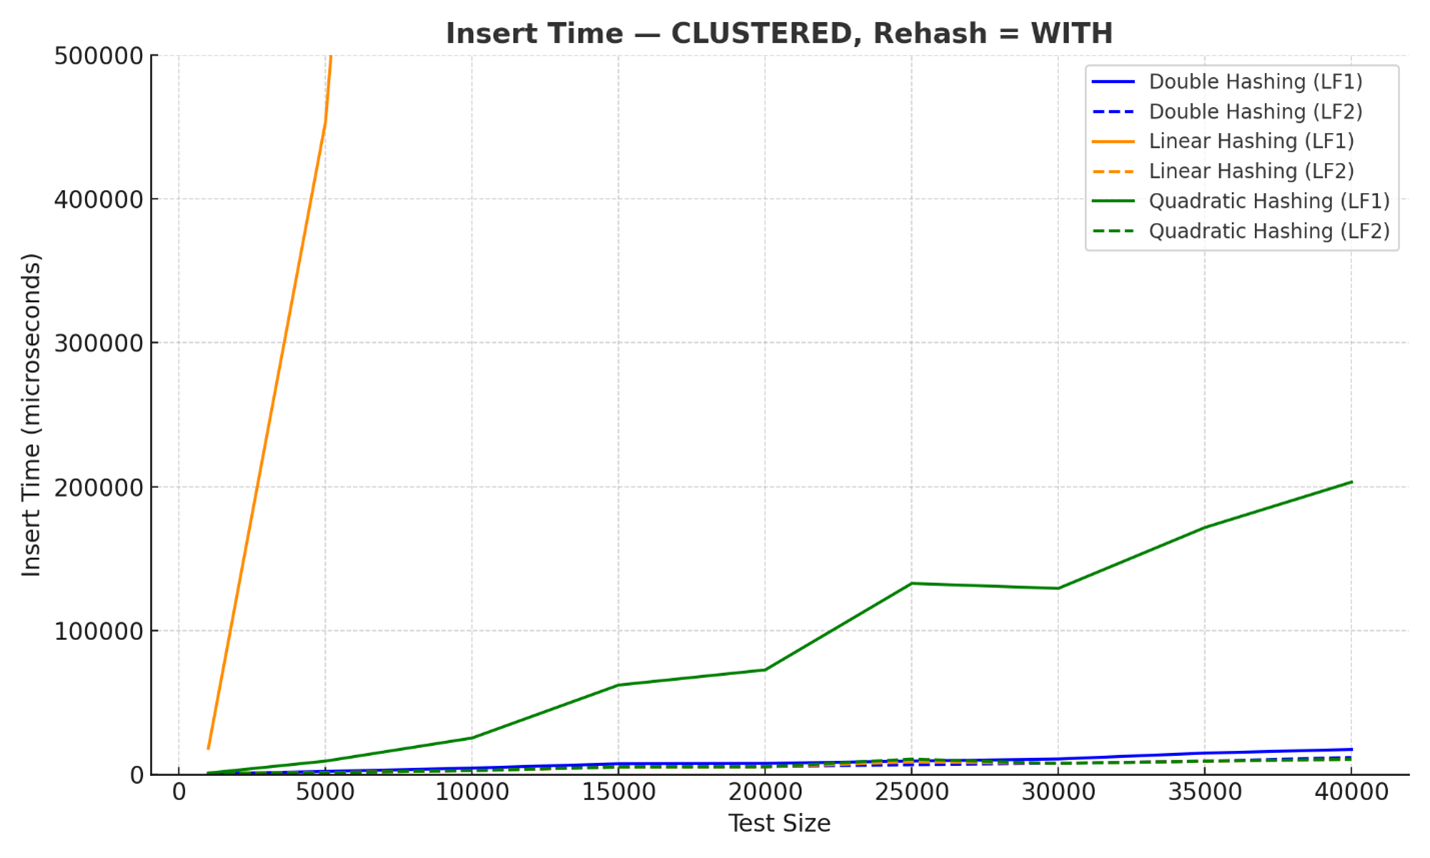
\includegraphics[width=0.8\textwidth]{clus_ins_hash.png}
    \caption{Đồ thị thời gian chèn theo số lượng phần tử của bảng băm có rehash với kiểu đầu vào phân cụm}
    \label{fig:flowchart}
\end{figure}

\begin{figure}[!ht]
    \centering
    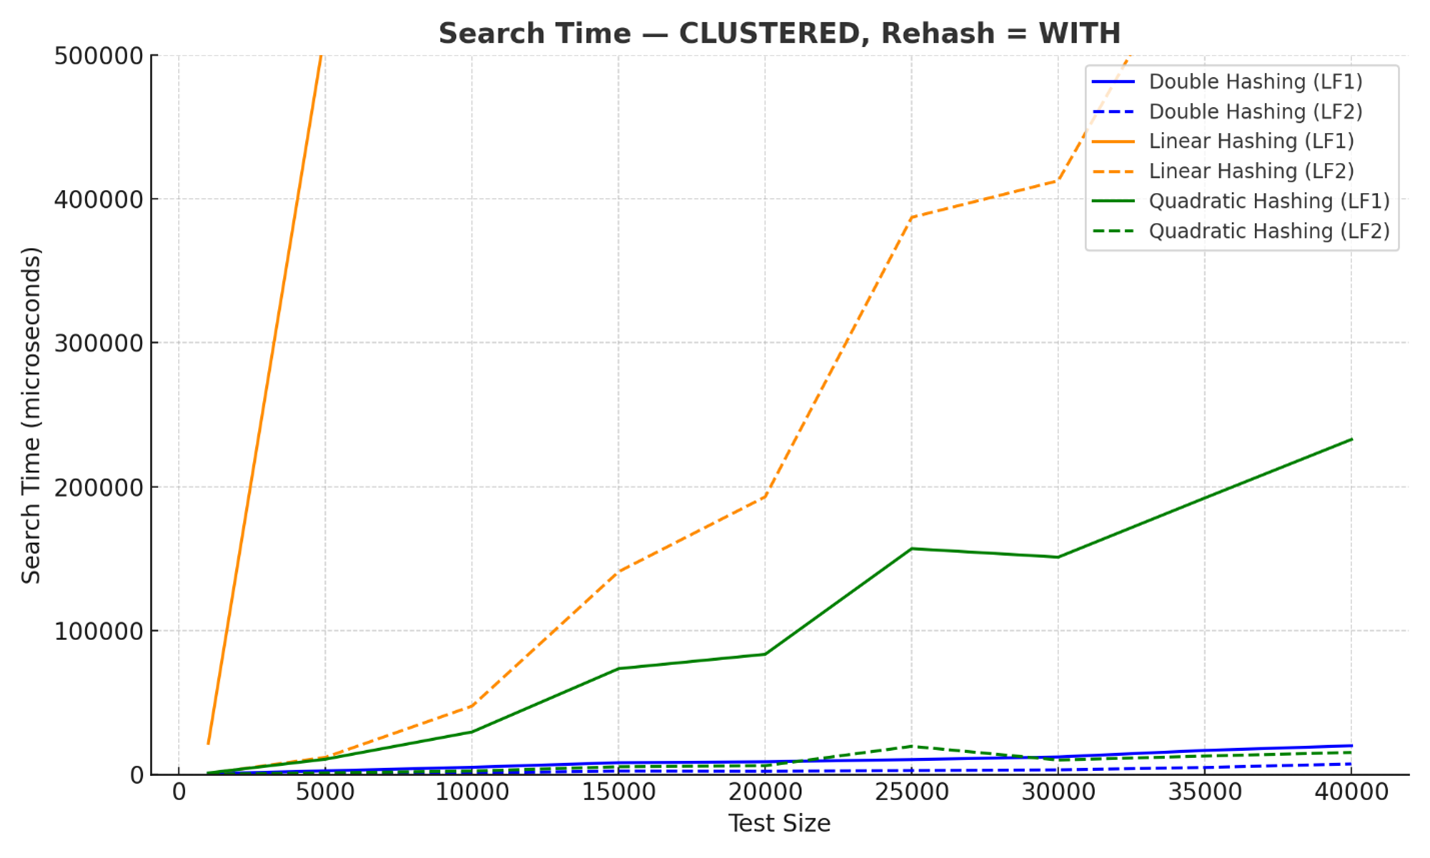
\includegraphics[width=0.8\textwidth]{clus_sear_hash.png}
    \caption{Đồ thị thời gian tìm theo số lượng phần tử của bảng băm có rehash với kiểu đầu vào phân cụm}
    \label{fig:flowchart}
\end{figure}

\begin{figure}[!ht]
    \centering
    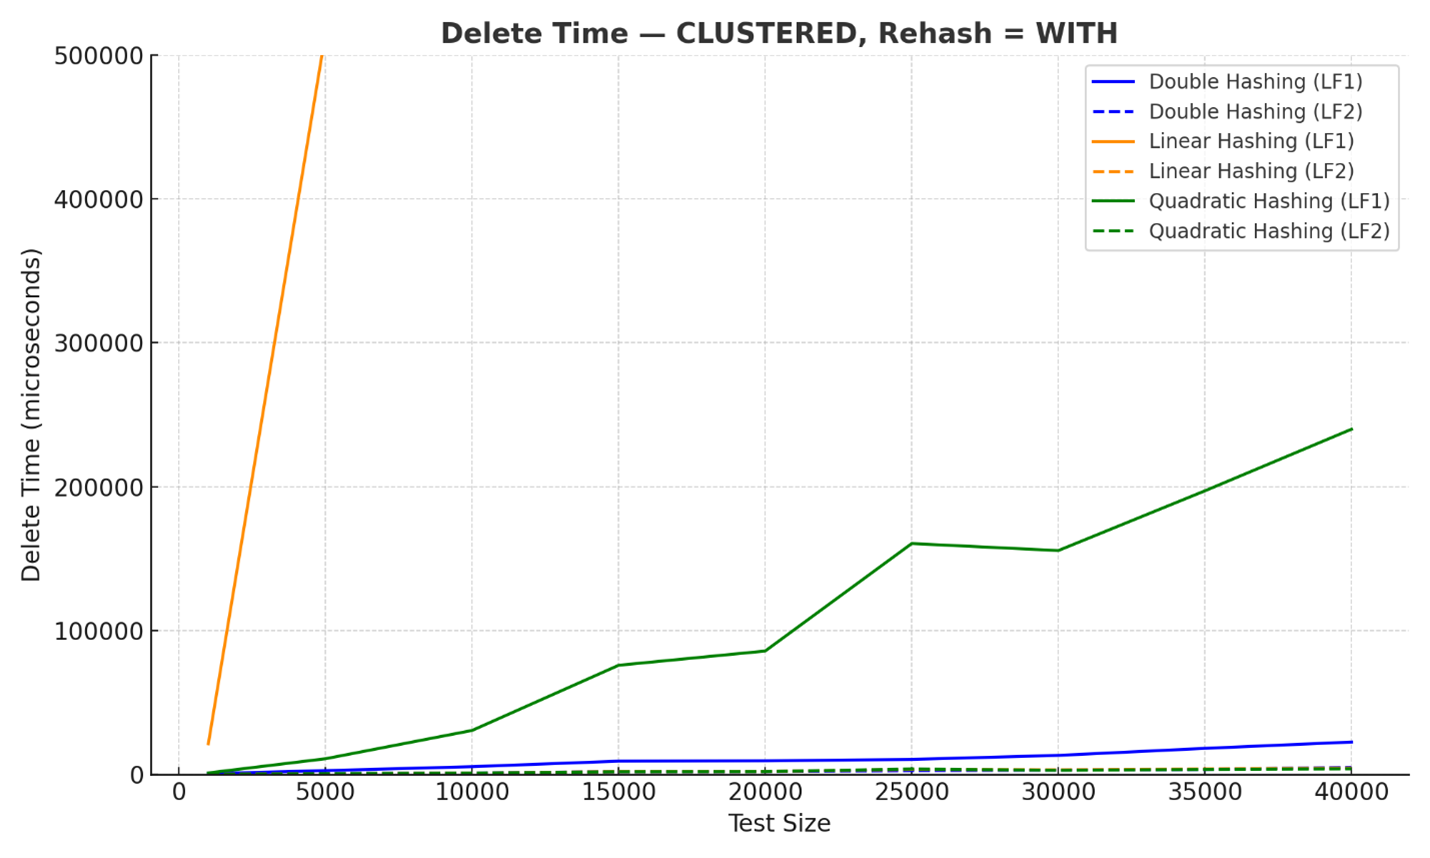
\includegraphics[width=0.8\textwidth]{clus_del_hash.png}
    \caption{Đồ thị thời gian xóa theo số lượng phần tử của bảng băm có rehash với kiểu đầu vào phân cụm}
    \label{fig:flowchart}
\end{figure}
\noindent \indent Ở hệ số tải thấp(LF1) Double Hashing vẫn có hiệu suất tốt nhất thời gian thực hiện các thao tác dưới 20000 mirco giây cho số lương khoá lớn nhất điều này càng rõ rệt khi kích thước dữ liệu càng lớn cụ thể :

-	Insert time ở 5000 khoá:

\hspace{1cm}+ Double Hashing mất 2688 mirco giây

\hspace{1cm}+ Quadratic Hashing mất 10167 mirco giây(gấp \textasciitilde 3,8 lần Double Hashing)

\hspace{1cm}+ Linear Hashing mất 535704 mirco giây(gấp \textasciitilde 200 lần Double Hashing)

-	Insert Time ở 20000 khoá:

\hspace{1cm}+ Double Hashing mất 7817 mirco giây(tăng \textasciitilde 2,9 lần)

\hspace{1cm}+ Quadratic Hashing mất 77478 mirco giây(tăng \textasciitilde 7,6 lần)

\hspace{1cm}+ Linear Hashing mất 7312906 mirco giây(tăng \textasciitilde 13 lần)

-	Khi số lượng khoá tăng lên khoảng 4 lần, thời gian thực hiện của Linear Hashing và Quadratic Hashing tăng lên đáng kể 13 lần(Linear),7,6 lần(Quadratic) nhưng Double Hashing chỉ tăng khoảng 2,9 lần.

-	Ở hệ số tải cao(LF2) cả 3 kiểu hashing có hiệu suất gần bằng nhau nhưng ở search time Linear Hashing có hiệu suất cực kì thấp.

\subsection*{4.3.3. Hiệu suất khi không rehash}

\begin{figure}[!ht]
    \centering
    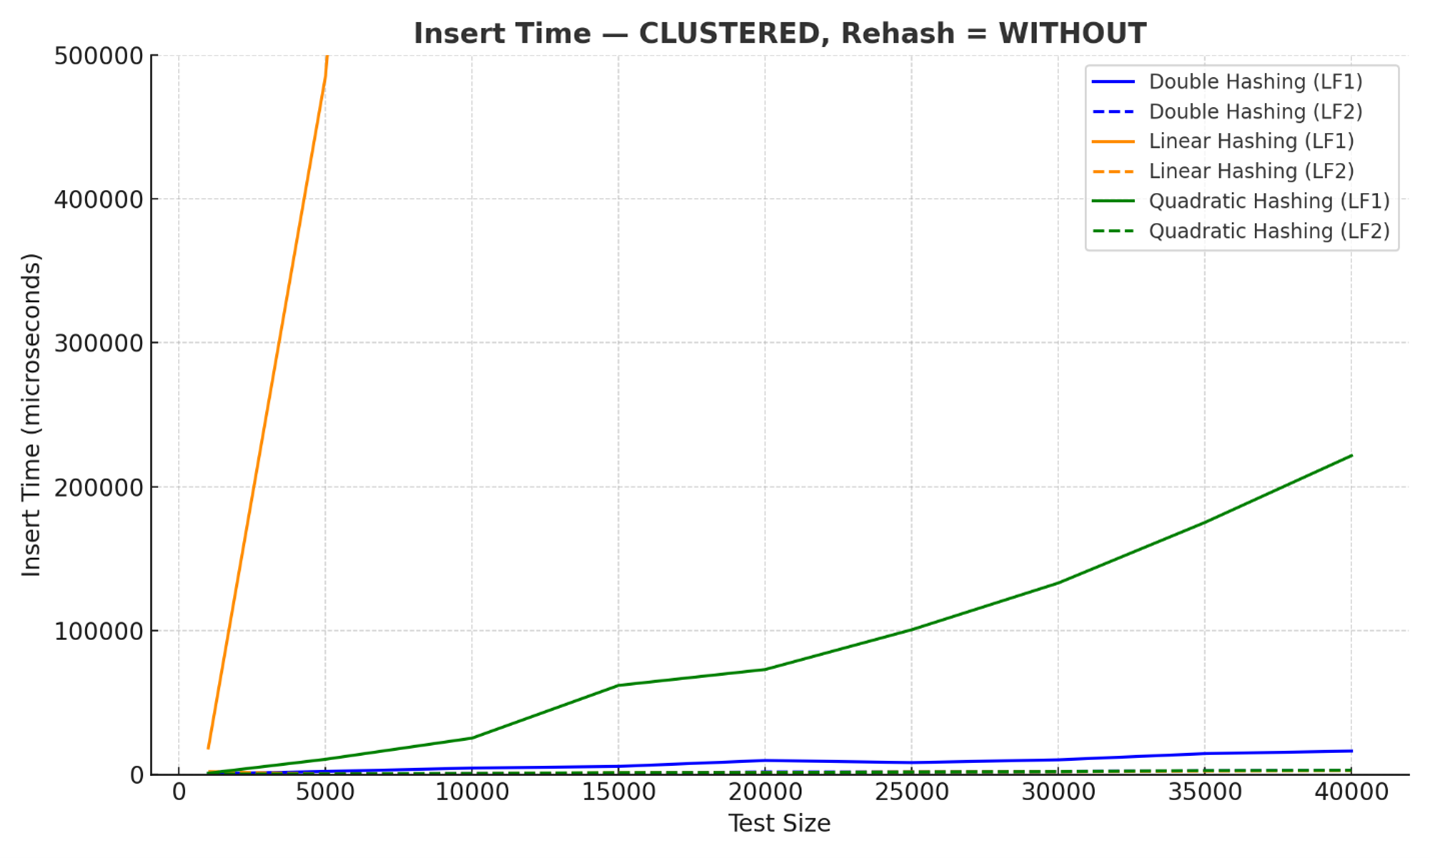
\includegraphics[width=0.8\textwidth]{clus_clus_not.png}
    \caption{Đồ thị thời gian chèn theo số lượng phần tử của bảng băm không có rehash với kiểu đầu vào phân cụm}
    \label{fig:flowchart}
\end{figure}

\begin{figure}[!ht]
    \centering
    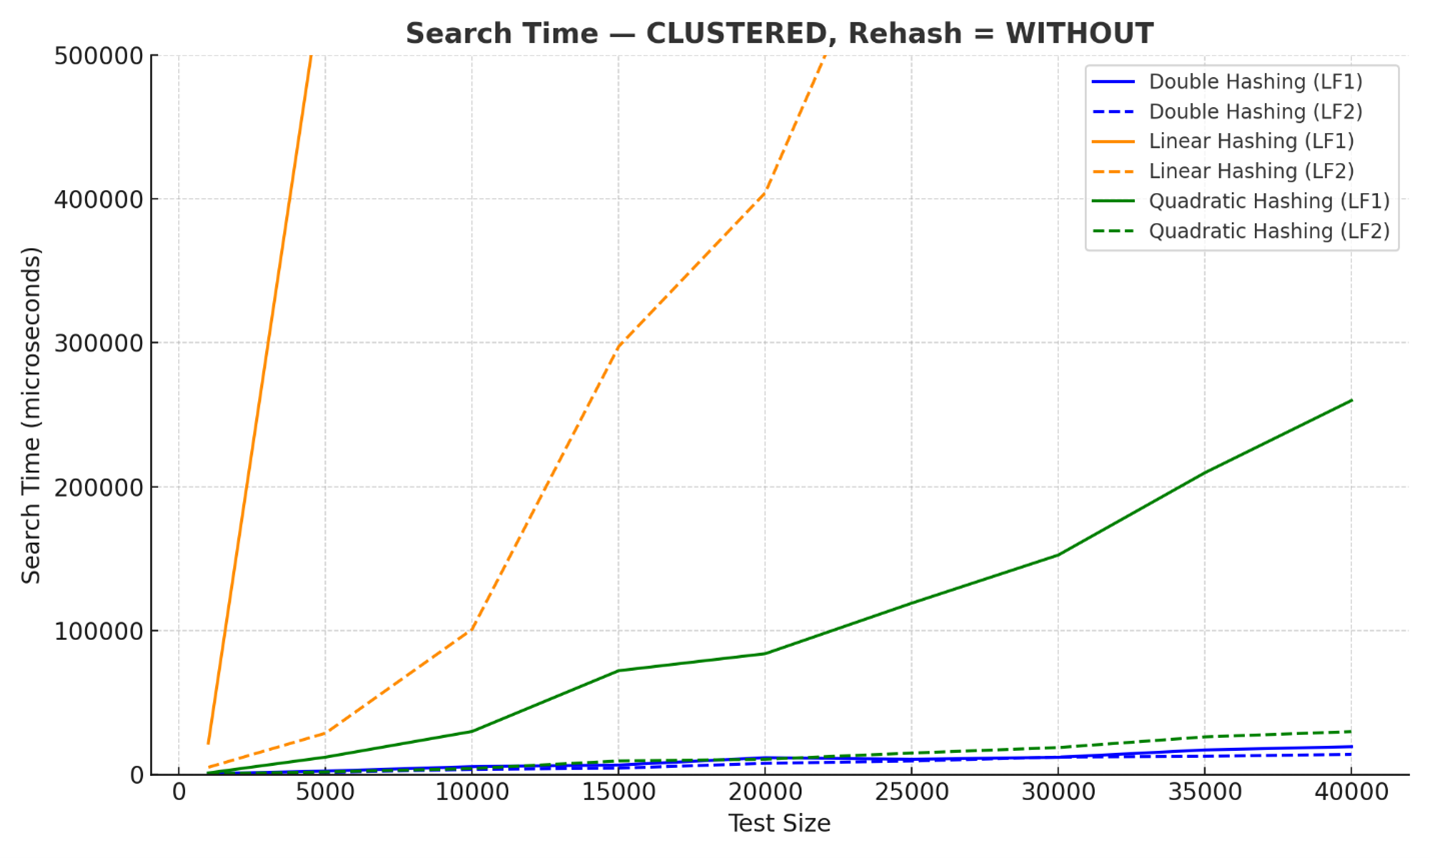
\includegraphics[width=0.8\textwidth]{clus_ser_not.png}
    \caption{Đồ thị thời gian tìm theo số lượng phần tử của bảng băm không có rehash với kiểu đầu vào phân cụm}
    \label{fig:flowchart}
\end{figure}

\begin{figure}[!ht]
    \centering
    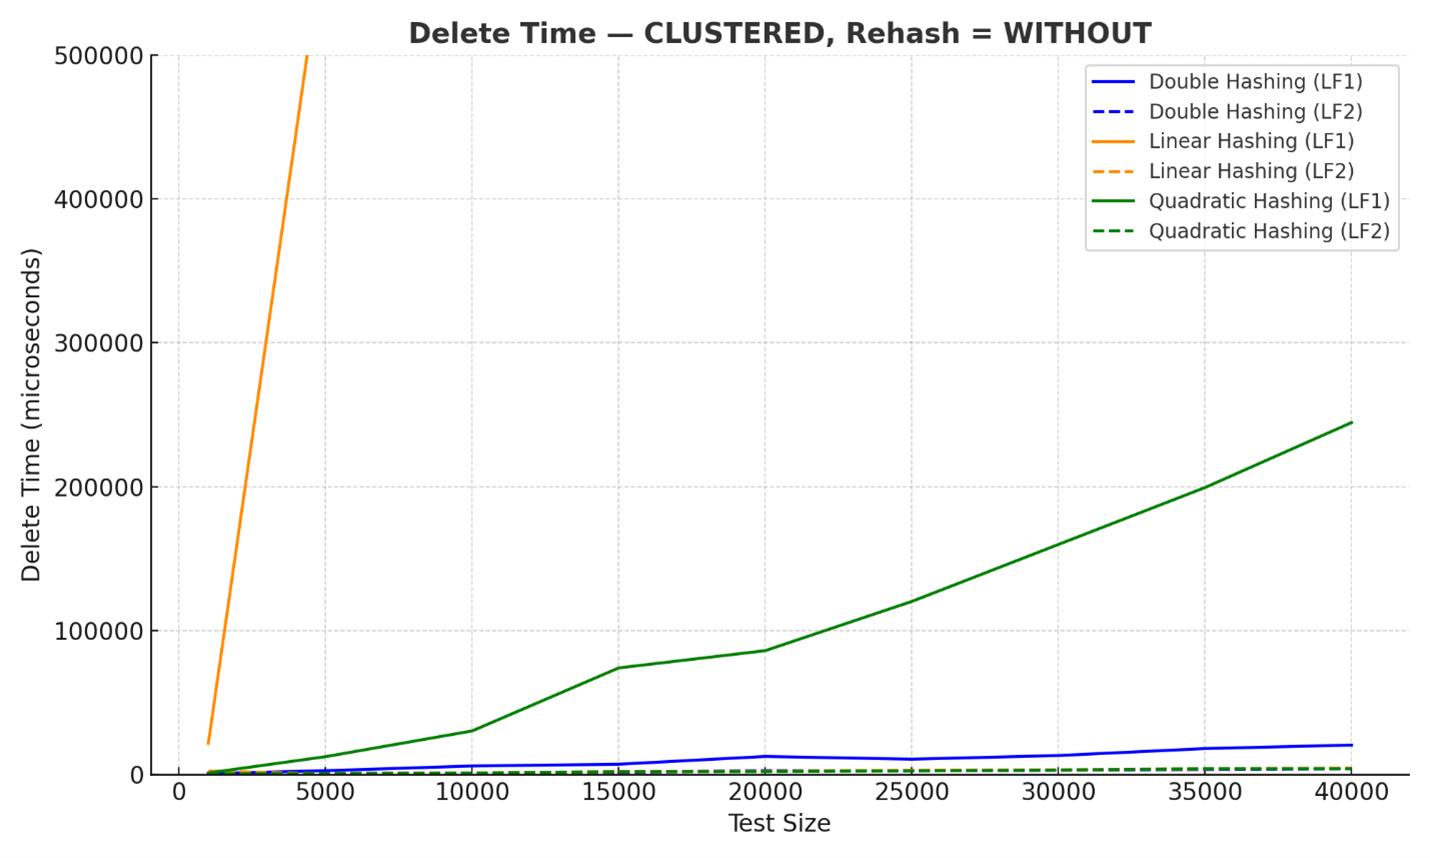
\includegraphics[width=0.8\textwidth]{clus_del_not.png}
    \caption{Đồ thị thời gian xóa theo số lượng phần tử của bảng băm không có rehash với kiểu đầu vào phân cụm}
    \label{fig:flowchart}
\end{figure}

-	Khi không rehash hầu hết thời gian thực hiện các thao tác có tăng lên nhưng không đáng kể,một số giảm.

-	Double Hashing dao động từ 5\% - 8\%

-	Linear Hashing dao động từ:3\% - 18\%,

-	Quadratic Hashing dao động từ:2\% - 29\%

\subsection*{4.3.4. Nhận xét}
\noindent \indent - Double Hashing là một phương án tối ưu dành cho cấu trúc dữ liệu bảng băm đặc biệt khi kích thước bảng lớn

    - Tuy nhiên Double Hashing cần đảm bảo hệ số tải(load factor) hợp lí để tối ưu hiệu suất và cách triển khai thường phức tạp hơn Linear và Quadratic.




\newpage
\chapter*{\centering{\MakeUppercase{Chương V. Kết luận và hướng phát triển}}}
\addcontentsline{toc}{chapter}{\textcolor{fitblue}{\MakeUppercase{Chương V. Kết luận và hướng phát triển}}}
\noindent \indent Chương trình benchmark này đã thực hiện việc so sánh hiệu suất của ba phương pháp dò tìm (Double Hashing, Linear Probing, và Quadratic Probing) trên bảng băm. Các bài kiểm tra được thực hiện với nhiều kích thước bảng khác nhau và với hai hệ số tải (0.5 và 0.9) để kiểm tra tác động của các yếu tố này đến hiệu suất của bảng băm.

Các kết quả đã chỉ ra rõ ràng các khác biệt về thời gian chèn (insert), tìm kiếm (search), và xóa (delete) giữa ba phương pháp dò tìm, đồng thời thống kê số lượng va chạm (collisions) và số lượng phép toán dò tìm (probes) trung bình trong mỗi lần chèn, tìm kiếm và xóa. Dữ liệu về độ dài cụm khoá (cluster length) cũng được thu thập để phân tích sự phân bố của các phần tử trong bảng băm sau các phép toán này. Mọi kết quả đã được ghi lại vào các tệp CSV để tiện cho việc phân tích sau này.
\section*{5.1. Hạn chế}
\addcontentsline{toc}{section}{{5.1. Hạn chế}}
    \noindent \indent - \textbf{Chạy thử nghiệm trên bộ dữ liệu giả lập}: Chương trình hiện đang sử dụng bộ dữ liệu giả lập cho các bài kiểm tra. Tuy nhiên, trong thực tế, bảng băm có thể gặp phải các tình huống phức tạp hơn như xung đột khóa dữ liệu thực tế, dữ liệu không đồng nhất hoặc không đều, điều này có thể ảnh hưởng đến hiệu suất của các phương pháp dò tìm.
    
    - \textbf{Không tối ưu hóa cho các trường hợp đặc biệt}: Các thử nghiệm chưa kiểm tra khả năng hoạt động của bảng băm trong những trường hợp đặc biệt như khóa trùng lặp quá nhiều, khóa có sự phân bố không đồng đều, hoặc bộ dữ liệu quá lớn.
    
    - \textbf{Chưa tối ưu hiệu suất mã nguồn}: Mặc dù chương trình đã thực hiện các phép toán cơ bản về thời gian và va chạm, nhưng có thể tối ưu thêm để tăng hiệu suất khi chạy với các bộ dữ liệu lớn.
    
    - \textbf{Chưa kiểm tra tính ổn định của bảng băm}: Việc tối ưu bảng băm sau mỗi lần va chạm chưa được kiểm tra nhiều trong chương trình. Các tính năng như tự động điều chỉnh kích thước bảng hoặc khả năng phản ứng với sự thay đổi của dữ liệu có thể chưa được xử lý tối ưu.

\section*{5.2. Đề xuất cải tiến, mở rộng}
\addcontentsline{toc}{section}{{5.2. Đề xuất cải tiến, mở rộng}}
    \subsection*{5.2.1. Tối ưu hóa bảng băm động}
        - Cần thử nghiệm với các chiến lược tối ưu hóa bảng băm, chẳng hạn như \textit{tự động điều chỉnh kích thước} bảng dựa trên các tham số như hệ số tải và số lượng va chạm.
        - Tích hợp các kỹ thuật như \textit{delayed rehashing} (tái tạo lại bảng khi cần thiết) hoặc \textit{adaptive resizing} để cải thiện hiệu suất trong các trường hợp dữ liệu lớn hoặc không đồng đều.
    
    \subsection*{5.2.2. Thử nghiệm với bộ dữ liệu thực tế}
        \noindent \indent Tiến hành các thử nghiệm với bộ dữ liệu thực tế để kiểm tra tính khả thi và hiệu quả của bảng băm trong các ứng dụng cụ thể như quản lý cơ sở dữ liệu, hệ thống tìm kiếm, hay các ứng dụng yêu cầu thời gian xử lý nhanh.
    
    \subsection*{5.2.3. Phân tích sự phân bố dữ liệu}
        \noindent \indent Phân tích các tình huống đặc biệt có thể xảy ra trong thực tế, chẳng hạn như phân bố dữ liệu không đều, các va chạm có thể xảy ra thường xuyên, và tính toán lại các chiến lược dựa trên các đặc điểm của dữ liệu đầu vào.
    
    \subsection*{5.2.4. Thử nghiệm với các phương pháp tối ưu hóa nâng cao}
    \noindent \indent Các kỹ thuật như \textit{hashing phân tán} (distributed hashing), \textit{perfect hashing}, hoặc \textit{cuckoo hashing} có thể được nghiên cứu và áp dụng để cải thiện hiệu suất của bảng băm trong các tình huống cụ thể.
    
    \subsection*{5.2.5. Tăng cường khả năng quản lý bộ nhớ}
        \noindent \indent Xử lý vấn đề bộ nhớ tốt hơn, đặc biệt khi làm việc với các bảng băm lớn. Tìm cách tối ưu việc cấp phát và giải phóng bộ nhớ để tránh các vấn đề về hiệu suất khi chạy chương trình với lượng dữ liệu lớn.
    
    \subsection*{5.2.6. Tích hợp nhiều chiến lược kiểm tra và phân tích sâu hơn}
        \noindent \indent Bổ sung khả năng phân tích các chiến lược dò tìm nâng cao, kết hợp với các tính toán thêm về thời gian hoạt động và phân tích dữ liệu nhằm tối ưu hóa hơn nữa các thao tác với bảng băm.
    
    \subsection*{5.2.7. Tích hợp giao diện người dùng (UI)}
        \noindent \indent Tạo một giao diện người dùng đơn giản, cho phép người dùng nhập vào các tham số thử nghiệm và nhận kết quả nhanh chóng. Giao diện này có thể giúp dễ dàng so sánh các kết quả và quyết định phương pháp dò tìm tối ưu cho các trường hợp cụ thể.

Với \textbf{những hướng phát triển} này, chương trình sẽ không chỉ hữu ích trong việc benchmark mà còn có thể ứng dụng rộng rãi trong các hệ thống thực tế, đảm bảo tính khả thi và tối ưu trong quá trình triển khai.

\newpage
\phantomsection
\addcontentsline{toc}{chapter}{\textcolor{fitblue}{\MakeUppercase{Tài liệu tham khảo}}}
\begin{thebibliography}{9}

\bibitem{luhn1953}
Luhn, H. P. (1953). A system for automatic keyword assignment. \textit{IBM Journal of Research and Development}.

\bibitem{knuth1998}
Knuth, D. E. (1998). \textit{The Art of Computer Programming}, Vol. 3: \textit{Sorting and Searching} (2nd ed.). Addison-Wesley.

\bibitem{carter1979}
Carter, L., \& Wegman, M. N. (1979). Universal classes of hash functions. \textit{Journal of Computer and System Sciences}, 18(2), 143–154.

\bibitem{brent1973}
Brent, R. P. (1973). Reducing the retrieval time of scatter storage techniques. \textit{Communications of the ACM}, 16(2), 105–109.

\bibitem{cormen2009}
Cormen, T. H., Leiserson, C. E., Rivest, R. L., \& Stein, C. (2009). \textit{Introduction to Algorithms} (3rd ed.). MIT Press.

\bibitem{weiss2012}
Weiss, M. A. (2012). \textit{Data Structures and Algorithm Analysis in C++} (4th ed.). Pearson.

\bibitem{khan2019}
Khan, M. A., Qureshi, M. A., \& Iqbal, T. (2019). Evaluation of Hashing Techniques for High Load Environments. \textit{International Journal of Computer Applications}, 180(32), 1–6.

\end{thebibliography}


\end{document}
